\documentclass[openany]{book}

    \usepackage[breakable]{tcolorbox}
    \usepackage{parskip} % Stop auto-indenting (to mimic markdown behaviour)
    \usepackage{blindtext}
    \usepackage[utf8]{inputenc}
    

    % Basic figure setup, for now with no caption control since it's done
    % automatically by Pandoc (which extracts ![](path) syntax from Markdown).
    \usepackage{minted}
    \usepackage{graphicx}
    \usepackage{svg}
    % Keep aspect ratio if custom image width or height is specified
    \setkeys{Gin}{keepaspectratio}
    % Maintain compatibility with old templates. Remove in nbconvert 6.0
    \let\Oldincludegraphics\includegraphics
    % Ensure that by default, figures have no caption (until we provide a
    % proper Figure object with a Caption API and a way to capture that
    % in the conversion process - todo).
    \usepackage{caption}
    \DeclareCaptionFormat{nocaption}{}
    \captionsetup{format=nocaption,aboveskip=0pt,belowskip=0pt}

    \usepackage{float}
    \floatplacement{figure}{H} % forces figures to be placed at the correct location
    \usepackage{xcolor} % Allow colors to be defined
    \usepackage{enumerate} % Needed for markdown enumerations to work
    \usepackage{geometry} % Used to adjust the document margins
    \usepackage{amsmath} % Equations
    \usepackage{amssymb} % Equations
    \usepackage{textcomp} % defines textquotesingle
    % Hack from http://tex.stackexchange.com/a/47451/13684:
    \AtBeginDocument{%
        \def\PYZsq{\textquotesingle}% Upright quotes in Pygmentized code
    }
    \usepackage{upquote} % Upright quotes for verbatim code
    \usepackage{eurosym} % defines \euro

    \usepackage{iftex}
    \ifPDFTeX
        \usepackage[T1]{fontenc}
        \IfFileExists{alphabeta.sty}{
              \usepackage{alphabeta}
          }{
              \usepackage[mathletters]{ucs}
              \usepackage[utf8x]{inputenc}
          }
    \else
        \usepackage{fontspec}
        \usepackage{unicode-math}
    \fi

    \usepackage{fancyvrb} % verbatim replacement that allows latex
    \usepackage{grffile} % extends the file name processing of package graphics
                         % to support a larger range
    \makeatletter % fix for old versions of grffile with XeLaTeX
    \@ifpackagelater{grffile}{2019/11/01}
    {
      % Do nothing on new versions
    }
    {
      \def\Gread@@xetex#1{%
        \IfFileExists{"\Gin@base".bb}%
        {\Gread@eps{\Gin@base.bb}}%
        {\Gread@@xetex@aux#1}%
      }
    }
    \makeatother
    \usepackage[Export]{adjustbox} % Used to constrain images to a maximum size
    \adjustboxset{max size={0.9\linewidth}{0.9\paperheight}}

    % The hyperref package gives us a pdf with properly built
    % internal navigation ('pdf bookmarks' for the table of contents,
    % internal cross-reference links, web links for URLs, etc.)
    \usepackage{hyperref}
    % The default LaTeX title has an obnoxious amount of whitespace. By default,
    % titling removes some of it. It also provides customization options.
    \usepackage{titling}
    \usepackage{longtable} % longtable support required by pandoc >1.10
    \usepackage{booktabs}  % table support for pandoc > 1.12.2
    \usepackage{array}     % table support for pandoc >= 2.11.3
    \usepackage{calc}      % table minipage width calculation for pandoc >= 2.11.1
    \usepackage[inline]{enumitem} % IRkernel/repr support (it uses the enumerate* environment)
    \usepackage[normalem]{ulem} % ulem is needed to support strikethroughs (\sout)
                                % normalem makes italics be italics, not underlines
    \usepackage{soul}      % strikethrough (\st) support for pandoc >= 3.0.0
    \usepackage{mathrsfs}
    

    
    % Colors for the hyperref package
    \definecolor{urlcolor}{rgb}{0,.145,.698}
    \definecolor{linkcolor}{rgb}{.71,0.21,0.01}
    \definecolor{citecolor}{rgb}{.12,.54,.11}

    % ANSI colors
    \definecolor{ansi-black}{HTML}{3E424D}
    \definecolor{ansi-black-intense}{HTML}{282C36}
    \definecolor{ansi-red}{HTML}{E75C58}
    \definecolor{ansi-red-intense}{HTML}{B22B31}
    \definecolor{ansi-green}{HTML}{00A250}
    \definecolor{ansi-green-intense}{HTML}{007427}
    \definecolor{ansi-yellow}{HTML}{DDB62B}
    \definecolor{ansi-yellow-intense}{HTML}{B27D12}
    \definecolor{ansi-blue}{HTML}{208FFB}
    \definecolor{ansi-blue-intense}{HTML}{0065CA}
    \definecolor{ansi-magenta}{HTML}{D160C4}
    \definecolor{ansi-magenta-intense}{HTML}{A03196}
    \definecolor{ansi-cyan}{HTML}{60C6C8}
    \definecolor{ansi-cyan-intense}{HTML}{258F8F}
    \definecolor{ansi-white}{HTML}{C5C1B4}
    \definecolor{ansi-white-intense}{HTML}{A1A6B2}
    \definecolor{ansi-default-inverse-fg}{HTML}{FFFFFF}
    \definecolor{ansi-default-inverse-bg}{HTML}{000000}

    % common color for the border for error outputs.
    \definecolor{outerrorbackground}{HTML}{FFDFDF}

    % commands and environments needed by pandoc snippets
    % extracted from the output of `pandoc -s`
    \providecommand{\tightlist}{%
      \setlength{\itemsep}{0pt}\setlength{\parskip}{0pt}}
    \DefineVerbatimEnvironment{Highlighting}{Verbatim}{commandchars=\\\{\}}
    % Add ',fontsize=\small' for more characters per line
    \newenvironment{Shaded}{}{}
    \newcommand{\KeywordTok}[1]{\textcolor[rgb]{0.00,0.44,0.13}{\textbf{{#1}}}}
    \newcommand{\DataTypeTok}[1]{\textcolor[rgb]{0.56,0.13,0.00}{{#1}}}
    \newcommand{\DecValTok}[1]{\textcolor[rgb]{0.25,0.63,0.44}{{#1}}}
    \newcommand{\BaseNTok}[1]{\textcolor[rgb]{0.25,0.63,0.44}{{#1}}}
    \newcommand{\FloatTok}[1]{\textcolor[rgb]{0.25,0.63,0.44}{{#1}}}
    \newcommand{\CharTok}[1]{\textcolor[rgb]{0.25,0.44,0.63}{{#1}}}
    \newcommand{\StringTok}[1]{\textcolor[rgb]{0.25,0.44,0.63}{{#1}}}
    \newcommand{\CommentTok}[1]{\textcolor[rgb]{0.38,0.63,0.69}{\textit{{#1}}}}
    \newcommand{\OtherTok}[1]{\textcolor[rgb]{0.00,0.44,0.13}{{#1}}}
    \newcommand{\AlertTok}[1]{\textcolor[rgb]{1.00,0.00,0.00}{\textbf{{#1}}}}
    \newcommand{\FunctionTok}[1]{\textcolor[rgb]{0.02,0.16,0.49}{{#1}}}
    \newcommand{\RegionMarkerTok}[1]{{#1}}
    \newcommand{\ErrorTok}[1]{\textcolor[rgb]{1.00,0.00,0.00}{\textbf{{#1}}}}
    \newcommand{\NormalTok}[1]{{#1}}

    % Additional commands for more recent versions of Pandoc
    \newcommand{\ConstantTok}[1]{\textcolor[rgb]{0.53,0.00,0.00}{{#1}}}
    \newcommand{\SpecialCharTok}[1]{\textcolor[rgb]{0.25,0.44,0.63}{{#1}}}
    \newcommand{\VerbatimStringTok}[1]{\textcolor[rgb]{0.25,0.44,0.63}{{#1}}}
    \newcommand{\SpecialStringTok}[1]{\textcolor[rgb]{0.73,0.40,0.53}{{#1}}}
    \newcommand{\ImportTok}[1]{{#1}}
    \newcommand{\DocumentationTok}[1]{\textcolor[rgb]{0.73,0.13,0.13}{\textit{{#1}}}}
    \newcommand{\AnnotationTok}[1]{\textcolor[rgb]{0.38,0.63,0.69}{\textbf{\textit{{#1}}}}}
    \newcommand{\CommentVarTok}[1]{\textcolor[rgb]{0.38,0.63,0.69}{\textbf{\textit{{#1}}}}}
    \newcommand{\VariableTok}[1]{\textcolor[rgb]{0.10,0.09,0.49}{{#1}}}
    \newcommand{\ControlFlowTok}[1]{\textcolor[rgb]{0.00,0.44,0.13}{\textbf{{#1}}}}
    \newcommand{\OperatorTok}[1]{\textcolor[rgb]{0.40,0.40,0.40}{{#1}}}
    \newcommand{\BuiltInTok}[1]{{#1}}
    \newcommand{\ExtensionTok}[1]{{#1}}
    \newcommand{\PreprocessorTok}[1]{\textcolor[rgb]{0.74,0.48,0.00}{{#1}}}
    \newcommand{\AttributeTok}[1]{\textcolor[rgb]{0.49,0.56,0.16}{{#1}}}
    \newcommand{\InformationTok}[1]{\textcolor[rgb]{0.38,0.63,0.69}{\textbf{\textit{{#1}}}}}
    \newcommand{\WarningTok}[1]{\textcolor[rgb]{0.38,0.63,0.69}{\textbf{\textit{{#1}}}}}
    \makeatletter
    \newsavebox\pandoc@box
    \newcommand*\pandocbounded[1]{%
      \sbox\pandoc@box{#1}%
      % scaling factors for width and height
      \Gscale@div\@tempa\textheight{\dimexpr\ht\pandoc@box+\dp\pandoc@box\relax}%
      \Gscale@div\@tempb\linewidth{\wd\pandoc@box}%
      % select the smaller of both
      \ifdim\@tempb\p@<\@tempa\p@
        \let\@tempa\@tempb
      \fi
      % scaling accordingly (\@tempa < 1)
      \ifdim\@tempa\p@<\p@
        \scalebox{\@tempa}{\usebox\pandoc@box}%
      % scaling not needed, use as it is
      \else
        \usebox{\pandoc@box}%
      \fi
    }
    \makeatother

    % Define a nice break command that doesn't care if a line doesn't already
    % exist.
    \def\br{\hspace*{\fill} \\* }
    % Math Jax compatibility definitions
    \def\gt{>}
    \def\lt{<}
    \let\Oldtex\TeX
    \let\Oldlatex\LaTeX
    \renewcommand{\TeX}{\textrm{\Oldtex}}
    \renewcommand{\LaTeX}{\textrm{\Oldlatex}}
    % Document parameters
    % Document title
    \title{Machine Learning Visualized}
    \author{Gavin Hung}
    
    
% Pygments definitions
\makeatletter
\def\PY@reset{\let\PY@it=\relax \let\PY@bf=\relax%
    \let\PY@ul=\relax \let\PY@tc=\relax%
    \let\PY@bc=\relax \let\PY@ff=\relax}
\def\PY@tok#1{\csname PY@tok@#1\endcsname}
\def\PY@toks#1+{\ifx\relax#1\empty\else%
    \PY@tok{#1}\expandafter\PY@toks\fi}
\def\PY@do#1{\PY@bc{\PY@tc{\PY@ul{%
    \PY@it{\PY@bf{\PY@ff{#1}}}}}}}
\def\PY#1#2{\PY@reset\PY@toks#1+\relax+\PY@do{#2}}

\@namedef{PY@tok@w}{\def\PY@tc##1{\textcolor[rgb]{0.73,0.73,0.73}{##1}}}
\@namedef{PY@tok@c}{\let\PY@it=\textit\def\PY@tc##1{\textcolor[rgb]{0.24,0.48,0.48}{##1}}}
\@namedef{PY@tok@cp}{\def\PY@tc##1{\textcolor[rgb]{0.61,0.40,0.00}{##1}}}
\@namedef{PY@tok@k}{\let\PY@bf=\textbf\def\PY@tc##1{\textcolor[rgb]{0.00,0.50,0.00}{##1}}}
\@namedef{PY@tok@kp}{\def\PY@tc##1{\textcolor[rgb]{0.00,0.50,0.00}{##1}}}
\@namedef{PY@tok@kt}{\def\PY@tc##1{\textcolor[rgb]{0.69,0.00,0.25}{##1}}}
\@namedef{PY@tok@o}{\def\PY@tc##1{\textcolor[rgb]{0.40,0.40,0.40}{##1}}}
\@namedef{PY@tok@ow}{\let\PY@bf=\textbf\def\PY@tc##1{\textcolor[rgb]{0.67,0.13,1.00}{##1}}}
\@namedef{PY@tok@nb}{\def\PY@tc##1{\textcolor[rgb]{0.00,0.50,0.00}{##1}}}
\@namedef{PY@tok@nf}{\def\PY@tc##1{\textcolor[rgb]{0.00,0.00,1.00}{##1}}}
\@namedef{PY@tok@nc}{\let\PY@bf=\textbf\def\PY@tc##1{\textcolor[rgb]{0.00,0.00,1.00}{##1}}}
\@namedef{PY@tok@nn}{\let\PY@bf=\textbf\def\PY@tc##1{\textcolor[rgb]{0.00,0.00,1.00}{##1}}}
\@namedef{PY@tok@ne}{\let\PY@bf=\textbf\def\PY@tc##1{\textcolor[rgb]{0.80,0.25,0.22}{##1}}}
\@namedef{PY@tok@nv}{\def\PY@tc##1{\textcolor[rgb]{0.10,0.09,0.49}{##1}}}
\@namedef{PY@tok@no}{\def\PY@tc##1{\textcolor[rgb]{0.53,0.00,0.00}{##1}}}
\@namedef{PY@tok@nl}{\def\PY@tc##1{\textcolor[rgb]{0.46,0.46,0.00}{##1}}}
\@namedef{PY@tok@ni}{\let\PY@bf=\textbf\def\PY@tc##1{\textcolor[rgb]{0.44,0.44,0.44}{##1}}}
\@namedef{PY@tok@na}{\def\PY@tc##1{\textcolor[rgb]{0.41,0.47,0.13}{##1}}}
\@namedef{PY@tok@nt}{\let\PY@bf=\textbf\def\PY@tc##1{\textcolor[rgb]{0.00,0.50,0.00}{##1}}}
\@namedef{PY@tok@nd}{\def\PY@tc##1{\textcolor[rgb]{0.67,0.13,1.00}{##1}}}
\@namedef{PY@tok@s}{\def\PY@tc##1{\textcolor[rgb]{0.73,0.13,0.13}{##1}}}
\@namedef{PY@tok@sd}{\let\PY@it=\textit\def\PY@tc##1{\textcolor[rgb]{0.73,0.13,0.13}{##1}}}
\@namedef{PY@tok@si}{\let\PY@bf=\textbf\def\PY@tc##1{\textcolor[rgb]{0.64,0.35,0.47}{##1}}}
\@namedef{PY@tok@se}{\let\PY@bf=\textbf\def\PY@tc##1{\textcolor[rgb]{0.67,0.36,0.12}{##1}}}
\@namedef{PY@tok@sr}{\def\PY@tc##1{\textcolor[rgb]{0.64,0.35,0.47}{##1}}}
\@namedef{PY@tok@ss}{\def\PY@tc##1{\textcolor[rgb]{0.10,0.09,0.49}{##1}}}
\@namedef{PY@tok@sx}{\def\PY@tc##1{\textcolor[rgb]{0.00,0.50,0.00}{##1}}}
\@namedef{PY@tok@m}{\def\PY@tc##1{\textcolor[rgb]{0.40,0.40,0.40}{##1}}}
\@namedef{PY@tok@gh}{\let\PY@bf=\textbf\def\PY@tc##1{\textcolor[rgb]{0.00,0.00,0.50}{##1}}}
\@namedef{PY@tok@gu}{\let\PY@bf=\textbf\def\PY@tc##1{\textcolor[rgb]{0.50,0.00,0.50}{##1}}}
\@namedef{PY@tok@gd}{\def\PY@tc##1{\textcolor[rgb]{0.63,0.00,0.00}{##1}}}
\@namedef{PY@tok@gi}{\def\PY@tc##1{\textcolor[rgb]{0.00,0.52,0.00}{##1}}}
\@namedef{PY@tok@gr}{\def\PY@tc##1{\textcolor[rgb]{0.89,0.00,0.00}{##1}}}
\@namedef{PY@tok@ge}{\let\PY@it=\textit}
\@namedef{PY@tok@gs}{\let\PY@bf=\textbf}
\@namedef{PY@tok@ges}{\let\PY@bf=\textbf\let\PY@it=\textit}
\@namedef{PY@tok@gp}{\let\PY@bf=\textbf\def\PY@tc##1{\textcolor[rgb]{0.00,0.00,0.50}{##1}}}
\@namedef{PY@tok@go}{\def\PY@tc##1{\textcolor[rgb]{0.44,0.44,0.44}{##1}}}
\@namedef{PY@tok@gt}{\def\PY@tc##1{\textcolor[rgb]{0.00,0.27,0.87}{##1}}}
\@namedef{PY@tok@err}{\def\PY@bc##1{{\setlength{\fboxsep}{\string -\fboxrule}\fcolorbox[rgb]{1.00,0.00,0.00}{1,1,1}{\strut ##1}}}}
\@namedef{PY@tok@kc}{\let\PY@bf=\textbf\def\PY@tc##1{\textcolor[rgb]{0.00,0.50,0.00}{##1}}}
\@namedef{PY@tok@kd}{\let\PY@bf=\textbf\def\PY@tc##1{\textcolor[rgb]{0.00,0.50,0.00}{##1}}}
\@namedef{PY@tok@kn}{\let\PY@bf=\textbf\def\PY@tc##1{\textcolor[rgb]{0.00,0.50,0.00}{##1}}}
\@namedef{PY@tok@kr}{\let\PY@bf=\textbf\def\PY@tc##1{\textcolor[rgb]{0.00,0.50,0.00}{##1}}}
\@namedef{PY@tok@bp}{\def\PY@tc##1{\textcolor[rgb]{0.00,0.50,0.00}{##1}}}
\@namedef{PY@tok@fm}{\def\PY@tc##1{\textcolor[rgb]{0.00,0.00,1.00}{##1}}}
\@namedef{PY@tok@vc}{\def\PY@tc##1{\textcolor[rgb]{0.10,0.09,0.49}{##1}}}
\@namedef{PY@tok@vg}{\def\PY@tc##1{\textcolor[rgb]{0.10,0.09,0.49}{##1}}}
\@namedef{PY@tok@vi}{\def\PY@tc##1{\textcolor[rgb]{0.10,0.09,0.49}{##1}}}
\@namedef{PY@tok@vm}{\def\PY@tc##1{\textcolor[rgb]{0.10,0.09,0.49}{##1}}}
\@namedef{PY@tok@sa}{\def\PY@tc##1{\textcolor[rgb]{0.73,0.13,0.13}{##1}}}
\@namedef{PY@tok@sb}{\def\PY@tc##1{\textcolor[rgb]{0.73,0.13,0.13}{##1}}}
\@namedef{PY@tok@sc}{\def\PY@tc##1{\textcolor[rgb]{0.73,0.13,0.13}{##1}}}
\@namedef{PY@tok@dl}{\def\PY@tc##1{\textcolor[rgb]{0.73,0.13,0.13}{##1}}}
\@namedef{PY@tok@s2}{\def\PY@tc##1{\textcolor[rgb]{0.73,0.13,0.13}{##1}}}
\@namedef{PY@tok@sh}{\def\PY@tc##1{\textcolor[rgb]{0.73,0.13,0.13}{##1}}}
\@namedef{PY@tok@s1}{\def\PY@tc##1{\textcolor[rgb]{0.73,0.13,0.13}{##1}}}
\@namedef{PY@tok@mb}{\def\PY@tc##1{\textcolor[rgb]{0.40,0.40,0.40}{##1}}}
\@namedef{PY@tok@mf}{\def\PY@tc##1{\textcolor[rgb]{0.40,0.40,0.40}{##1}}}
\@namedef{PY@tok@mh}{\def\PY@tc##1{\textcolor[rgb]{0.40,0.40,0.40}{##1}}}
\@namedef{PY@tok@mi}{\def\PY@tc##1{\textcolor[rgb]{0.40,0.40,0.40}{##1}}}
\@namedef{PY@tok@il}{\def\PY@tc##1{\textcolor[rgb]{0.40,0.40,0.40}{##1}}}
\@namedef{PY@tok@mo}{\def\PY@tc##1{\textcolor[rgb]{0.40,0.40,0.40}{##1}}}
\@namedef{PY@tok@ch}{\let\PY@it=\textit\def\PY@tc##1{\textcolor[rgb]{0.24,0.48,0.48}{##1}}}
\@namedef{PY@tok@cm}{\let\PY@it=\textit\def\PY@tc##1{\textcolor[rgb]{0.24,0.48,0.48}{##1}}}
\@namedef{PY@tok@cpf}{\let\PY@it=\textit\def\PY@tc##1{\textcolor[rgb]{0.24,0.48,0.48}{##1}}}
\@namedef{PY@tok@c1}{\let\PY@it=\textit\def\PY@tc##1{\textcolor[rgb]{0.24,0.48,0.48}{##1}}}
\@namedef{PY@tok@cs}{\let\PY@it=\textit\def\PY@tc##1{\textcolor[rgb]{0.24,0.48,0.48}{##1}}}

\def\PYZbs{\char`\\}
\def\PYZus{\char`\_}
\def\PYZob{\char`\{}
\def\PYZcb{\char`\}}
\def\PYZca{\char`\^}
\def\PYZam{\char`\&}
\def\PYZlt{\char`\<}
\def\PYZgt{\char`\>}
\def\PYZsh{\char`\#}
\def\PYZpc{\char`\%}
\def\PYZdl{\char`\$}
\def\PYZhy{\char`\-}
\def\PYZsq{\char`\'}
\def\PYZdq{\char`\"}
\def\PYZti{\char`\~}
% for compatibility with earlier versions
\def\PYZat{@}
\def\PYZlb{[}
\def\PYZrb{]}
\makeatother


    % For linebreaks inside Verbatim environment from package fancyvrb.
    \makeatletter
        \newbox\Wrappedcontinuationbox
        \newbox\Wrappedvisiblespacebox
        \newcommand*\Wrappedvisiblespace {\textcolor{red}{\textvisiblespace}}
        \newcommand*\Wrappedcontinuationsymbol {\textcolor{red}{\llap{\tiny$\m@th\hookrightarrow$}}}
        \newcommand*\Wrappedcontinuationindent {3ex }
        \newcommand*\Wrappedafterbreak {\kern\Wrappedcontinuationindent\copy\Wrappedcontinuationbox}
        % Take advantage of the already applied Pygments mark-up to insert
        % potential linebreaks for TeX processing.
        %        {, <, #, %, $, ' and ": go to next line.
        %        _, }, ^, &, >, - and ~: stay at end of broken line.
        % Use of \textquotesingle for straight quote.
        \newcommand*\Wrappedbreaksatspecials {%
            \def\PYGZus{\discretionary{\char`\_}{\Wrappedafterbreak}{\char`\_}}%
            \def\PYGZob{\discretionary{}{\Wrappedafterbreak\char`\{}{\char`\{}}%
            \def\PYGZcb{\discretionary{\char`\}}{\Wrappedafterbreak}{\char`\}}}%
            \def\PYGZca{\discretionary{\char`\^}{\Wrappedafterbreak}{\char`\^}}%
            \def\PYGZam{\discretionary{\char`\&}{\Wrappedafterbreak}{\char`\&}}%
            \def\PYGZlt{\discretionary{}{\Wrappedafterbreak\char`\<}{\char`\<}}%
            \def\PYGZgt{\discretionary{\char`\>}{\Wrappedafterbreak}{\char`\>}}%
            \def\PYGZsh{\discretionary{}{\Wrappedafterbreak\char`\#}{\char`\#}}%
            \def\PYGZpc{\discretionary{}{\Wrappedafterbreak\char`\%}{\char`\%}}%
            \def\PYGZdl{\discretionary{}{\Wrappedafterbreak\char`\$}{\char`\$}}%
            \def\PYGZhy{\discretionary{\char`\-}{\Wrappedafterbreak}{\char`\-}}%
            \def\PYGZsq{\discretionary{}{\Wrappedafterbreak\textquotesingle}{\textquotesingle}}%
            \def\PYGZdq{\discretionary{}{\Wrappedafterbreak\char`\"}{\char`\"}}%
            \def\PYGZti{\discretionary{\char`\~}{\Wrappedafterbreak}{\char`\~}}%
        }
        % Some characters . , ; ? ! / are not pygmentized.
        % This macro makes them "active" and they will insert potential linebreaks
        \newcommand*\Wrappedbreaksatpunct {%
            \lccode`\~`\.\lowercase{\def~}{\discretionary{\hbox{\char`\.}}{\Wrappedafterbreak}{\hbox{\char`\.}}}%
            \lccode`\~`\,\lowercase{\def~}{\discretionary{\hbox{\char`\,}}{\Wrappedafterbreak}{\hbox{\char`\,}}}%
            \lccode`\~`\;\lowercase{\def~}{\discretionary{\hbox{\char`\;}}{\Wrappedafterbreak}{\hbox{\char`\;}}}%
            \lccode`\~`\:\lowercase{\def~}{\discretionary{\hbox{\char`\:}}{\Wrappedafterbreak}{\hbox{\char`\:}}}%
            \lccode`\~`\?\lowercase{\def~}{\discretionary{\hbox{\char`\?}}{\Wrappedafterbreak}{\hbox{\char`\?}}}%
            \lccode`\~`\!\lowercase{\def~}{\discretionary{\hbox{\char`\!}}{\Wrappedafterbreak}{\hbox{\char`\!}}}%
            \lccode`\~`\/\lowercase{\def~}{\discretionary{\hbox{\char`\/}}{\Wrappedafterbreak}{\hbox{\char`\/}}}%
            \catcode`\.\active
            \catcode`\,\active
            \catcode`\;\active
            \catcode`\:\active
            \catcode`\?\active
            \catcode`\!\active
            \catcode`\/\active
            \lccode`\~`\~
        }
    \makeatother

    \let\OriginalVerbatim=\Verbatim
    \makeatletter
    \renewcommand{\Verbatim}[1][1]{%
        %\parskip\z@skip
        \sbox\Wrappedcontinuationbox {\Wrappedcontinuationsymbol}%
        \sbox\Wrappedvisiblespacebox {\FV@SetupFont\Wrappedvisiblespace}%
        \def\FancyVerbFormatLine ##1{\hsize\linewidth
            \vtop{\raggedright\hyphenpenalty\z@\exhyphenpenalty\z@
                \doublehyphendemerits\z@\finalhyphendemerits\z@
                \strut ##1\strut}%
        }%
        % If the linebreak is at a space, the latter will be displayed as visible
        % space at end of first line, and a continuation symbol starts next line.
        % Stretch/shrink are however usually zero for typewriter font.
        \def\FV@Space {%
            \nobreak\hskip\z@ plus\fontdimen3\font minus\fontdimen4\font
            \discretionary{\copy\Wrappedvisiblespacebox}{\Wrappedafterbreak}
            {\kern\fontdimen2\font}%
        }%

        % Allow breaks at special characters using \PYG... macros.
        \Wrappedbreaksatspecials
        % Breaks at punctuation characters . , ; ? ! and / need catcode=\active
        \OriginalVerbatim[#1,codes*=\Wrappedbreaksatpunct]%
    }
    \makeatother

    % Exact colors from NB
    \definecolor{incolor}{HTML}{303F9F}
    \definecolor{outcolor}{HTML}{D84315}
    \definecolor{cellborder}{HTML}{CFCFCF}
    \definecolor{cellbackground}{HTML}{F7F7F7}

    % prompt
    \makeatletter
    \newcommand{\boxspacing}{\kern\kvtcb@left@rule\kern\kvtcb@boxsep}
    \makeatother
    \newcommand{\prompt}[4]{
        {\ttfamily\llap{{\color{#2}[#3]:\hspace{3pt}#4}}\vspace{-\baselineskip}}
    }
    

    
    % Prevent overflowing lines due to hard-to-break entities
    \sloppy
    % Setup hyperref package
    \hypersetup{
      breaklinks=true,  % so long urls are correctly broken across lines
      colorlinks=true,
      urlcolor=urlcolor,
      linkcolor=linkcolor,
      citecolor=citecolor,
      }
    % Slightly bigger margins than the latex defaults
    
    \geometry{verbose,tmargin=1in,bmargin=1in,lmargin=1in,rmargin=1in}
    
    

\begin{document}

\maketitle

\tableofcontents
    
NumPy citation: \cite{harris2020array}

PyTorch citation: \cite{paszke2017automatic}
    
    \section{Gradient Descent}\label{gradient-descent}

Gradient Descent is an algorithm that finds the local extrema of a
function. This is applicable to machine learning, because we want to
find the optimal parameters that minimize our loss function. In machine
learning, loss functions quantify the amount of error between the
predicted values from a machine learning model and the actual expected
values. In this notebook, we will perform linear regression by using
gradient descent to find the optimal slope and y-intercept.

    \subsection{Training Dataset}\label{training-dataset}

    Importing the libraries

\begin{tcolorbox}
\tiny
\begin{verbatim}
import numpy as np

import matplotlib.pyplot as plt
import scienceplots
from IPython.display import display, Latex, Image

from celluloid import Camera

np.random.seed(0)
plt.style.use(["science", "no-latex"])
\end{verbatim}
\end{tcolorbox}

    Let's look at the training dataset. We will use columns 2 and 4 of the
txt file. The linear regression model will find the optimal slope and
y-intercept to fit the data.

\begin{tcolorbox}
\tiny
\begin{verbatim}
fname = "REGRESSION-gradientDescent-data.txt"
x, y = np.loadtxt(fname, delimiter=",", unpack=True, skiprows=1, usecols=(2, 4))

fig = plt.figure()
ax = fig.add_subplot()
ax.scatter(x, y, color="#1f77b4", marker="o", alpha=0.25)
\end{verbatim}
\end{tcolorbox}
        
    \begin{center}
    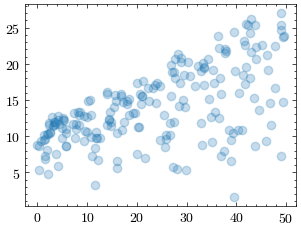
\includegraphics[width=\textwidth]{combined_files/combined_5_1.png}
    \end{center}
    { \hspace*{\fill} \\}
    
    \subsection{Loss Function: Mean Squared
Error}\label{loss-function-mean-squared-error}

    For the linear regression model, the predicted value \(\hat{y}\) is the
dot product of the weight and x input vectors plus a bias term

\(\hat{y} = w x + b\)

We will use the mean squared error function as our loss function.

\begin{align*}
MSE &= \frac{1}{n} \sum_{i=1}^{n}(y_{i}-\hat{y})^2 \\
&= \frac{1}{n} \sum_{i=1}^{n}(y_{i}-(w x_{i} + b))^2
\end{align*}

    \subsection{Loss Function Gradient}\label{loss-function-gradient}

    \begin{tcolorbox}
\tiny
\begin{verbatim}
def mse_loss(x, y, w, b):
    return np.mean(np.square(y - (w * x + b)))
\end{verbatim}
\end{tcolorbox}

    In each epoch of gradient descent, a parameter is updated by subtracting
the product of the gradient of the function and the learning rate
(\(lr\)). The learning rate controls how much the parameters should
change. Small learning rates are precise, but are slow. Large learning
rates are fast, but may prevent the model from finding the local
extrema.

\begin{align*}
X_{n+1} = X_n - lr * \frac{\partial}{\partial X} f(X_n)
\end{align*}

Since we are finding the optimal slope (\(w\)) and y-intercept (\(b\))
for our linear regression model, we must find the partial derivatives of
the loss function with respect to \(w\) and \(b\).

    \subsection{Loss Function in Terms of
W}\label{loss-function-in-terms-of-w}

    Loss function with respect to \(w\):

\begin{align*}
\frac{\partial }{\partial w} \left( MSE \right) &= \frac{\partial }{\partial w}[\frac{1}{n} \sum_{i=1}^{n}(y_{i}-(w x_{i} + b))^2] \\
&= \frac{1}{n} \sum_{i=1}^{n} \frac{\partial }{\partial w}[(y_{i}-(w x_{i} + b))^2] \\
&= \frac{2}{n} \sum_{i=1}^{n} (y_{i}-(w x_{i} + b))\frac{\partial }{\partial w}[y_{i}-(w x_{i} + b)] \\
&= \frac{2}{n} \sum_{i=1}^{n} (y_{i}-(w x_{i} + b))(-x_{i}) \\ 
&= -\frac{2}{n} \sum_{i=1}^{n}x_{i}(y_{i}-(w x_{i} + b))
\end{align*}

\begin{tcolorbox}
\tiny
\begin{verbatim}
def mse_loss_dw(x, y, w, b):
    return -2 * np.mean(x * (y - (w * x + b)))
\end{verbatim}
\end{tcolorbox}

    \subsection{Loss Function in Terms of
b}\label{loss-function-in-terms-of-b}

    Loss function with respect to \(b\):

\begin{align*}
\frac{\partial}{\partial b} \left( MSE \right) &=  \frac{\partial }{\partial b}[\frac{1}{n} \sum_{i=1}^{n}(y_{i}-(w x_{i} + b))^2] \\
&= \frac{1}{n} \sum_{i=1}^{n} \frac{\partial }{\partial b}[(y_{i}-(w x_{i} + b))^2] \\
&= \frac{2}{n} \sum_{i=1}^{n} (y_{i}-(w x_{i} + b))\frac{\partial }{\partial b}[y_{i}-(w x_{i} + b)] \\
&= \frac{2}{n} \sum_{i=1}^{n} (y_{i}-(w x_{i} + b))(-1) \\ 
&= -\frac{2}{n} \sum_{i=1}^{n} (y_{i}-(w x_{i} + b))
\end{align*}

\begin{tcolorbox}
\tiny
\begin{verbatim}
def mse_loss_db(x, y, w, b):
    return -2 * np.mean(y - (w * x + b))
\end{verbatim}
\end{tcolorbox}

    \subsection{Training the Linear Regression
Model}\label{training-the-linear-regression-model}

    Let's define a function that uses the gradient algorithm to update the
parameters of the loss function. The function uses the gradient
functions we derived earlier.

General Gradient Descent Equation:
\[
X_{n+1} = X_n - \text{lr} \cdot \frac{\partial}{\partial X} f(X_n)
\]

Bias Gradient Descent:

\begin{align*}
b &= b - \eta \frac{\partial}{\partial b} [L(\vec{w}, b)] \\
&= b - \eta [-\frac{2}{n} \sum_{i=1}^{n} (y_{i}-(w x_{i} + b))]
\end{align*}

    Weights Gradient Descent:

\begin{align*}
b &= b - \eta \frac{\partial}{\partial b} [L(\vec{w}, b)] \\
&= b - \eta [-\frac{2}{n} \sum_{i=1}^{n}x_{i}(y_{i}-(w x_{i} + b))]
\end{align*}

\begin{tcolorbox}
\tiny
\begin{verbatim}
def update_w_and_b(x, y, w, b, learning_rate):
    # update w and b
    w = w - mse_loss_dw(x, y, w, b) * learning_rate
    b = b - mse_loss_db(x, y, w, b) * learning_rate

    return w, b
\end{verbatim}
\end{tcolorbox}

    \subsection{Graphing functions}\label{graphing-functions}

Let's define helper functions to plot the graphs.

\begin{tcolorbox}
\tiny
\begin{verbatim}
def create_plots():
    plt.ioff()
    fig = plt.figure(figsize=(16 / 9.0 * 4, 4 * 1), layout="constrained")
    fig.suptitle("Gradient Descent")
    ax0 = fig.add_subplot(1, 2, 1)
    ax0.set_xlabel("Spending", fontweight="normal")
    ax0.set_ylabel("Sales", fontweight="normal")
    ax0.set_title("Linear Regression")

    ax1 = fig.add_subplot(1, 2, 2, projection="3d")
    ax1.set_xlabel("Slope, w")
    ax1.set_ylabel("Intercept, b")
    ax1.set_zlabel("Error")
    ax1.set_title("Error")
    ax1.view_init(15, -35)

    camera = Camera(fig)
    return ax0, ax1, camera


def generate_error_range(x, y, N, w_max, b_max):
    w_range = np.arange(0, w_max, w_max / N)
    b_range = np.arange(0, b_max, b_max / N)
    w_range, b_range = np.meshgrid(w_range, b_range)
    w_range = w_range.flatten()
    b_range = b_range.flatten()

    error_range = np.array([])
    for i in range(min(w_range.shape[0], b_range.shape[0])):
        error_range = np.append(error_range, mse_loss(x, y, w_range[i], b_range[i]))

    return w_range, b_range, error_range
\end{verbatim}
\end{tcolorbox}

    \subsection{Training the model}\label{training-the-model}

The train function will update the parameters in each epoch and update
the visualization.

\begin{tcolorbox}
\tiny
\begin{verbatim}
def train(x, y, w0, b0, learning_rate, epochs, output_filename):
    w = w0
    b = b0

    ax0, ax1, camera = create_plots()
    loss_dims = 20
    w_max = 0.5
    b_max = 15
    w_range, b_range, error_range = generate_error_range(x, y, loss_dims, w_max, b_max)

    for e in range(epochs):
        w, b = update_w_and_b(x, y, w, b, learning_rate)
        if (
            (e == 0)
            or (e < 60 and e % 5 == 0)
            or (e < 3000 and e % 1000 == 0)
            or (e % 3000 == 0)
        ):
            # Plot the error given the current slope and y-intercept
            ax1.scatter(w_range, b_range, error_range, color="blue", alpha=0.05)
            ax1.scatter([w], [b], [mse_loss(x, y, w, b)], color="red", s=100)

            # Plot the linear regression lines
            ax0.scatter(x, y, color="#1f77b4", marker="o", alpha=0.25)
            X_plot = np.linspace(0, 50, 50)
            ax0.plot(X_plot, X_plot * w + b, color="black")

            # print the loss
            print("epoch: ", str(e), "loss: " + str(mse_loss(x, y, w, b)))
            camera.snap()

    animation = camera.animate()
    animation.save(output_filename, writer="pillow")
    plt.show()

    return w, b
\end{verbatim}
\end{tcolorbox}
    Let's train the linear regression model on a sample dataset.

\begin{tcolorbox}
\tiny
\begin{verbatim}
fname = "REGRESSION-gradientDescent-data.txt"
x, y = np.loadtxt(fname, delimiter=",", unpack=True, skiprows=1, usecols=(2, 4))
output_filename = "gradient_descent.gif"
train(x, y, 0.0, 0, 0.00005, 4000, output_filename)
\end{verbatim}
\end{tcolorbox}

    \begin{center}
    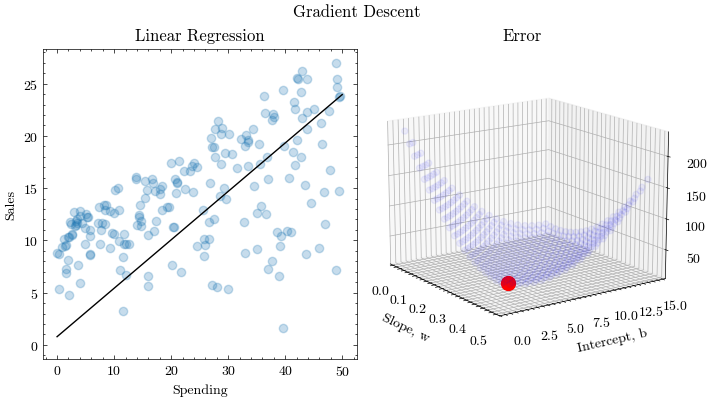
\includegraphics[width=\textwidth]{combined_files/combined_27_1.png}
    \end{center}
    { \hspace*{\fill} \\}
        
    \section{K-Means Clustering}\label{k-means-clustering}

This is an unsupervised clustering algorithm that assigns points to a
centroid. This is a quick way of grouping data points together and to
identify outliers. The downside of this algorithm is that it takes up a
lot of memory as everything has to be loaded in. However, it is very
easy to implement and has many use cases

    Import the libraries

\begin{tcolorbox}
\tiny
\begin{verbatim}
import numpy as np

import matplotlib.pyplot as plt
import scienceplots

from IPython.display import Image
from celluloid import Camera

np.random.seed(0)
plt.style.use(["science", "no-latex"])
\end{verbatim}
\end{tcolorbox}

    \subsection{Example Dataset}\label{example-dataset}

Let's generate a dataset of random points

\begin{tcolorbox}
\tiny
\begin{verbatim}
K = 12
w = 1200
h = 675
nums = 100

colors = np.random.rand(K, 3)

x = np.random.randint(0, w, size=nums)
y = np.random.randint(0, h, size=nums)
pts = np.column_stack((x, y))

# plot the points
fig = plt.figure()
ax = fig.add_subplot(111)

ax.scatter(x, y)
\end{verbatim}
\end{tcolorbox}
        
    \begin{center}
    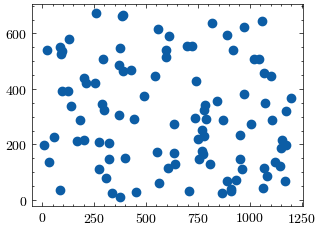
\includegraphics[width=\textwidth]{combined_files/combined_33_1.png}
    \end{center}
    { \hspace*{\fill} \\}
    
    \subsection{Distance Functions}\label{distance-functions}

When assigning points to centroids, we assign them to the closest
centroid. In order to quantify this, we need to state how we measure
distance. The following are 2 examples of distance functions.

Given point \(p1\) at \((x_1, y_1)\) and point \(p2\) at \((x_2, y_2)\),
we can develop the following distance functions

Euclidean Distance: \(\sqrt{(x_2-x_1)^2 + (y_2-y_1)^2}\)

Manhattan Distance: \(|x_2-x_1| + |y_2-y_1|\)

\begin{tcolorbox}
\tiny
\begin{verbatim}
def euclidean_distance(p1, p2):
    return np.sqrt((p1[0] - p2[0]) ** 2 + (p1[1] - p2[1]) ** 2)


def manhattan_distance(p1, p2):
    return abs(p1[0] - p2[0]) + abs(p1[1] - p2[1])
\end{verbatim}
\end{tcolorbox}

    \subsection{K Means Setup}\label{k-means-setup}

At the beginning, the centroids are initialized with random x and y values.

\begin{tcolorbox}
\tiny
\begin{verbatim}
centroids_x = np.random.randint(0, w, size=K)
centroids_y = np.random.randint(0, h, size=K)
centroids = np.column_stack((centroids_x, centroids_y))
\end{verbatim}
\end{tcolorbox}

    \subsection{Graphing Functions}\label{graphing-functions}

Create a helper function to create a plot with the sum of the distances
squared on the left and the centroids on the right. Also initialize
variables for the visualization, like the sum of the distances so far.

\begin{tcolorbox}
\tiny
\begin{verbatim}
def create_plots():
    fig, ax = plt.subplots(1, 3, figsize=(16 / 9.0 * 4, 4 * 1), layout="constrained")
    fig.suptitle("K-Means Clustering Unsupervised")

    ax[0].set_xlabel("K Clusters", fontweight="normal")
    ax[0].set_ylabel("Sum of Euclidean Distance Squared", fontweight="normal")
    ax[0].set_title("Elbow Method")

    ax[1].axis("off")
    ax[2].axis("off")

    ax[2] = fig.add_subplot(1, 2, 2)
    ax[2].set_xlabel("X")
    ax[2].set_ylabel("Y")
    ax[2].set_title("Centroids")

    camera = Camera(fig)
    return ax[0], ax[2], camera

boundary_div = 25
x_boundary_inc = int(w / boundary_div)
y_boundary_inc = int(h / boundary_div)

x_boundary = np.linspace(0, w, x_boundary_inc + 1)
y_boundary = np.linspace(0, h, y_boundary_inc + 1)
x_boundary, y_boundary = np.meshgrid(x_boundary, y_boundary)
colors_idx_boundary = np.random.randint(0, K, size=x_boundary.shape)

x_boundary_flat = x_boundary.flatten()
y_boundary_flat = y_boundary.flatten()

dists = np.zeros(K)
dists_idx = np.arange(1, K + 1)
\end{verbatim}
\end{tcolorbox}

    \subsection{Training the Model}\label{training-the-model}

Let's bring everything together. In this visualization, I show the
centroids with varying values of K, which is the total number of
centroids. For every value of K, I run the algorithm for a certain
number of epochs. At the start, centroids start at a random location on
the grid. In each epoch, points are assigned to the closest centroid.
Then, the next location of the centroid is the average x and y value of
all the points assigned to it in the previoius iteration.

\begin{tcolorbox}
\tiny
\begin{verbatim}
ax0, ax1, camera = create_plots()
epochs = 8

output_filename = "k_means.gif"

for k in range(1, K + 1):
    acc_dist_squared = 0
    for e in range(epochs):
        # Draw the boundaries
        for index in np.ndindex(x_boundary.shape):
            x = x_boundary[index]
            y = y_boundary[index]

            colors_idx_boundary[index] = 0
            min_group = 0
            # set min distance to largest possible distance initially
            min_dist = np.sqrt(w**2 + h**2)

            curr_pt = [x, y]
            curr_c = []
            for c in range(k):
                curr_c = centroids[c]

                dist = euclidean_distance(curr_pt, curr_c)
                if dist < min_dist:
                    min_dist = dist
                    min_group = c
            colors_idx_boundary[index] = min_group

        colors_boundary = colors[colors_idx_boundary.flatten()]
        ax1.scatter(
            x_boundary_flat, y_boundary_flat, c=colors_boundary, s=20, alpha=0.45
        )

        # Assign each point to a centroid
        groups = [[] for _ in range(k)]
        acc_dist_squared = 0
        for i in range(nums):
            min_group = 0
            # set min distance to largest possible distance initially
            min_dist = np.sqrt(w**2 + h**2)

            curr_pt = pts[i]
            curr_c = []
            for c in range(k):
                curr_c = centroids[c]

                dist = euclidean_distance(curr_pt, curr_c)
                if dist < min_dist:
                    min_dist = dist
                    min_group = c

            groups[min_group].append(curr_pt)
            acc_dist_squared += min_dist**2

        # Centroids
        for g in range(k):
            # Draw the centroids
            curr_centroid = centroids[g]
            curr_centroid = np.array([curr_centroid], dtype=np.int32)
            ax1.scatter(curr_centroid[:, 0], curr_centroid[:, 1], color=colors[g], s=8)

            group_pts = np.array(groups[g])
            if group_pts.size != 0:
                # Draw lines between points and the centroids
                pts_in_group = group_pts.shape[0]
                for i in range(pts_in_group):
                    group_pt = group_pts[i]
                    ax1.plot(
                        [group_pt[0], centroids[g][0]],
                        [group_pt[1], centroids[g][1]],
                        color=colors[g],
                        linewidth=2,
                        alpha=0.55,
                    )

                # Update the location of the centroids
                new_centroid = np.mean(group_pts, axis=0)
                centroids[g] = new_centroid
                new_centroid = np.array([new_centroid], dtype=np.int32)

        # Draw the points
        ax1.scatter(pts[:, 0], pts[:, 1], c="black", s=15, alpha=0.3)
        # Draw the Elbow Method graph
        if k - 2 > 0:
            ax0.plot(dists_idx[: k - 1], dists[: k - 1], color="red")
        camera.snap()
        # if e % 2 == 0:
        #     camera.snap()
        # else:
        #     ax0.clear()
        #     ax1.clear()

    acc_dist_squared /= nums
    dists[k - 1] = acc_dist_squared
    print(k-1, acc_dist_squared)

animation = camera.animate()
animation.save("k_means.gif", writer="pillow")
plt.close()
\end{verbatim}
\end{tcolorbox}
        
    \section{Principal Component
Analysis}\label{principal-component-analysis}

An important decision to make when training machine learning models is
the the features to use for the training dataset. Principal Component
Analysis allows you to see which features account for most of the
variance, simplifying the dataset to a smaller number of correlated
variables.

\begin{tcolorbox}
\tiny
\begin{verbatim}
import numpy as np

%matplotlib widget
import matplotlib.pyplot as plt
from mpl_toolkits.mplot3d import Axes3D
import scienceplots
from celluloid import Camera

from IPython.display import Image

np.random.seed(0)
plt.style.use(["science", "no-latex"])
\end{verbatim}
\end{tcolorbox}

    \subsection{Target Dataset}\label{target-dataset}

Let's generate a noisy list of points by generating points between a
start and end point and by adding random noise to each point

\begin{tcolorbox}
\tiny
\begin{verbatim}
def generate_noisy_hyperplane(num_points, start_pt, end_pt, noise=0.25):
    # create a plane from the start to the end point
    t = np.linspace(0.0 + noise, 1.0 - noise, num_points).reshape(-1, 1)
    points = start_pt + t * (end_pt - start_pt)

    # add noise to plane
    noise = np.random.normal(0, noise, size=(num_points, 3))
    points = points + noise

    return points


start_pt = np.array([-1, -1, -1])
end_pt = np.array([1, 1, 1])
X = generate_noisy_hyperplane(200, start_pt, end_pt)

# plot the points
fig = plt.figure()
ax = fig.add_subplot(111, projection="3d")
ax.scatter(X[:, 0], X[:, 1], X[:, 2], alpha=0.2, color="blue", label="Original Data")
plt.show()
\end{verbatim}
\end{tcolorbox}

    \begin{center}
    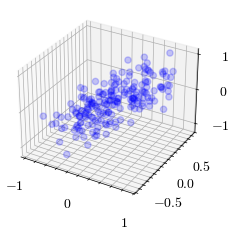
\includegraphics[width=\textwidth]{combined_files/combined_46_0.png}
    \end{center}
    { \hspace*{\fill} \\}
    
    \subsection{Eigenvectors and
Eigenvalues}\label{eigenvectors-and-eigenvalues}

When you multiply a matrix with its eigenvector, you get a multiple of
the eigenvector. The scalar multiple is the eigenvector's eigenvalue.
The process of finding the eigenvectors and eigenvalues of a matrix is
called Eigendecomposition.

\[A \vec{v} = \lambda \vec{v}\]

The scalar \(\lambda\) is the eigenvalue and the vector \(\vec{v}\) is
the corresponding eigenvector. The eigendecomposition typically involves
solving the determinant \(det(A - \lambda I) = 0\), where \(I\) is the
identity matrix.

Use numpy to quickly get the eigenvalues and eigenvectors of a matrix

\begin{tcolorbox}
\tiny
\begin{verbatim}
import numpy as np
mat = np.array([[4, -2],
                [1,  1]])
eig_vals, eig_vecs = np.linalg.eig(mat)
\end{verbatim}
\end{tcolorbox}

    \subsection{Lagrange Multipliers (Optimization with
constraints)}\label{lagrange-multipliers-optimization-with-constraints}

Recall from Multivariable Calculus that Lagrange Multipliers allow you
to find the extrema of a function \(f(x, y, z, ...)\) that is subject to
a constraint function \(g(x, y, z, ...)=0\).

The Lagrange Multipliers technique states that the solution of this
constrainted optimization problem is the solution to the following
system of equations:

\[\nabla L = 0\]

where

\[L(x, y, z, ... \lambda) = f(x, y, z, ... \lambda) - \lambda g(x, y, z, ... \lambda)\]

    \subsection{PCA Derivation (Eigendecomposition of Covariance
Matrix)}\label{pca-derivation-eigendecomposition-of-covariance-matrix}

Recall that our goal is to find the vectors \(v\) that account for most
of the variance.

Given input vector \(x_i\) and vector \(v\), we want to project every
input point to \(v\) in each dimension.

\[z_i = x_i^Tv\]

The variance is

\[(x_i^Tv)^2 = z_i^2\]

To find the maximum variance across all of the projections for the \(n\)
dimensions.

\begin{align*}
\max \sum_{i=1}^{n} (x_i^Tv)^2 &= \max \sum_{i=1}^{n} z_i^2 \\ 
&= \max z^Tz \\ 
&= \arg\max (xv)^Txv \\ 
\end{align*}

Since the ratios of the Principal Components is all that matters, let's
introduce the constaint that \[v^Tv = 1\]

    Solving the constrainted optimization with Lagrange Multipliers, we
define the Lagrangian function:

\[ L = \arg\max v^Tx^Txv - \lambda (v^Tv - 1)\]

Let's solve the Lagrangian function by solving \(\nabla L = 0\)

\begin{align*}
0 &= \frac{\partial L}{\partial v} \\ 
&= \frac{\partial}{\partial v}[v^Tx^Txv - \lambda (v^Tv - 1)]  \\ 
&= 2x^Txv - 2\lambda v  \\
&= x^Txv - \lambda v  \\
&= (x^Tx)v - \lambda v  \\
(x^Tx)v &= \lambda v  \\
\end{align*}

Given that \(x^Tx\) is the covariance of a matrix, we see that the
solution to PCA is simply the eigendecomposition of the covariance
matrix.

    \subsection{PCA Implementation}\label{pca-implementation}

To recap the two sections above, PCA consists of the following parts: 1.
Standard the input data by dividing the difference of the data and the
mean by the standard deviation. 2. Compute the covariance matrix of the
standardized input 3. Compute eigenvalues and eigenvectors of the
covariance matrix 4. To get the projected data, matrix multiply the
standardized input and the eigenvectors.

\begin{tcolorbox}
\tiny
\begin{verbatim}
def pca(X, dims):
    # subtract the mean to center the data and divide by standard deviation
    X_centered = (X - np.mean(X, axis=0)) / np.std(X, axis=0)

    # compute covariance matrix
    cov = np.cov(X_centered.T)

    # eigendecomposition of the covariance matrix
    # the eigenvectors are the principal components
    # the principal components are the columns of the eig_vecs matrix
    eig_vals, eig_vecs = np.linalg.eig(cov)

    # sort the eigenvalues and eigenvectors
    sorted_idx = np.argsort(eig_vals)[::-1]
    eig_vals = eig_vals[sorted_idx]
    eig_vecs = eig_vecs[:, sorted_idx]

    # perform dimensionality reduction using the computed principal components
    # if you want to reduce to K dimensions, simplify take the first K columns
    projected = X_centered @ eig_vecs

    # compute the variance of each dimension (column)
    pc_variances = [np.var(projected[:, i]) for i in range(dims)]

    return eig_vals, eig_vecs, projected, pc_variances
\end{verbatim}
\end{tcolorbox}

    \subsection{Graphing Functions}\label{graphing-functions}

Utility functions to create the visualizations

\begin{tcolorbox}
\tiny
\begin{verbatim}
def create_plots():
    fig = plt.figure(figsize=(16 / 9.0 * 4, 4 * 1))
    fig.suptitle("Principal Component Analysis")

    ax0 = fig.add_subplot(121, projection="3d")
    ax0.set_xlabel("X")
    ax0.set_ylabel("Y")
    ax0.set_zlabel("Z")
    ax0.set_title("PC Hyperplanes")
    ax0.view_init(17, -125, 2)
    ax0.set_xlim(-1, 1)
    ax0.set_ylim(-1, 1)
    ax0.set_zlim(-1, 1)
    ax0.tick_params(axis="both", which="both", length=0)

    ax1 = fig.add_subplot(122, projection="3d")
    ax1.set_xlabel("X")
    ax1.set_ylabel("Y")
    ax1.set_zlabel("Z")
    ax1.set_title("Projected Data")
    ax1.view_init(17, -125, 2)
    # ax1.set_xlim(-1, 1)
    # ax1.set_ylim(-1, 1)
    # ax1.set_zlim(-1, 1)
    ax1.tick_params(axis="both", which="both", length=0)
    # plt.axis('equal')

    camera = Camera(fig)
    return ax0, ax1, camera


def plot_hyperplane(ax, pc_vector, color="red", scaling=10, alpha=0.3):
    # Create a grid of points
    points = np.linspace(-1, 1, scaling)
    xx, yy = np.meshgrid(points, points)

    # the z value is the defined by the hyperplane from the principal component vector
    pc_vector /= np.linalg.norm(pc_vector)
    z = (-pc_vector[0] * xx - pc_vector[1] * yy) / pc_vector[2]

    ax.plot_surface(xx, yy, z, color=color, alpha=alpha)
\end{verbatim}
\end{tcolorbox}

    \subsection{Visualize PCA}\label{visualize-pca}

Given the derivation of PCA, let's visualize the projected data with
different values for the target dimension.

\begin{tcolorbox}
\tiny
\begin{verbatim}
def visualize_pca(X, dims, output_filename):
    ax0, ax1, camera = create_plots()
    colors = ["red", "green", "blue"]

    for dim in range(0, dims + 1):
        eig_vals, eig_vecs, projected, pc_variances = pca(X, dims)

        # plot the original data
        ax0.scatter(X[:, 0], X[:, 1], X[:, 2], color="blue", label="Original Data")

        # plot the pca hyperplanes
        for i in range(dim):
            plot_hyperplane(ax0, eig_vecs[:, i], color=colors[i])

        # plot the projected data from the principal components
        curr_projected = projected
        for i in range(dim, dims):
            if i < dims:
                curr_projected[:, i] = 0
        if dim != 0:
            ax1.scatter(
                curr_projected[:, 0],
                curr_projected[:, 1],
                curr_projected[:, 2],
                color="blue",
                label="Projected Data",
            )

        camera.snap()

    animation = camera.animate(interval=2000)
    animation.save(output_filename, writer="pillow")
    plt.show()

    eig_vals, eig_vecs, projected, pc_variances = pca(X, dims)

    print("variance percentage per principal component")
    variance_percentage = eig_vals / np.sum(eig_vals)
    for i, percentage in enumerate(variance_percentage):
        print(f"{i+1}th PC: {round(percentage*100, 2)}%")

    print("variance per principal component")
    for i, variance in enumerate(pc_variances):
        print(f"{i+1}th PC: {round(variance, 2)}")

    print("\nhyperplanes")
    for i in range(dim):
        print(f"hyperplane {i}: {eig_vecs[:, i]}")
\end{verbatim}
\end{tcolorbox}

\begin{tcolorbox}
\tiny
\begin{verbatim}
dims = 3
output_filename = "pca.gif"

visualize_pca(X, dims, output_filename)
\end{verbatim}
\end{tcolorbox}

    \begin{center}
    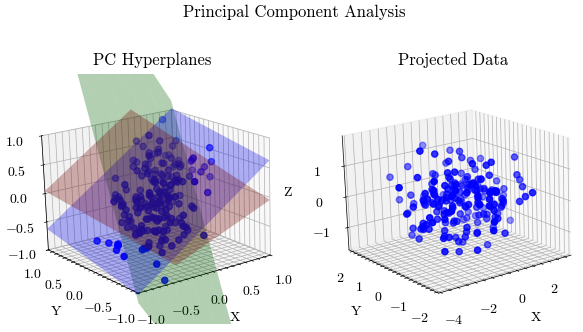
\includegraphics[width=\textwidth]{combined_files/combined_57_0.png}
    \end{center}
    { \hspace*{\fill} \\}

    \subsection{Scikit-Learn
Implementation}\label{scikit-learn-implementation}

As a check for correctness, let's compare our results with the PCA
module from scikit-learn.

Note: The sign of the values might not match exactly. They just need to
have the same ratios, which they do. Our implementation matches the one
from scikit-learn.

\begin{tcolorbox}
\tiny
\begin{verbatim}
from sklearn.decomposition import PCA
from sklearn.preprocessing import StandardScaler

scaler = StandardScaler()
X_centered = scaler.fit_transform(X)

pca = PCA(n_components=dims)
projected = pca.fit_transform(X_centered)
eig_vecs = pca.components_

print("\nhyperplanes")
for i in range(dims):
    print(f"hyperplane {i}: {eig_vecs[i]}")
\end{verbatim}
\end{tcolorbox}

    Let's also plot scikit's learn projected data. Our implementation seems
to match for the projected as well.

\begin{tcolorbox}
\tiny
\begin{verbatim}
fig = plt.figure()
ax = fig.add_subplot(111, projection="3d")
ax.scatter(projected[:, 0], projected[:, 1], projected[:, 2], alpha=0.2, color="blue", label="Projected Data")
plt.show()
\end{verbatim}
\end{tcolorbox}

    \begin{center}
    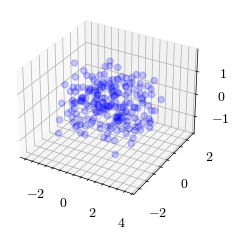
\includegraphics[width=\textwidth]{combined_files/combined_62_0.png}
    \end{center}
    { \hspace*{\fill} \\}
    
    \section{Logistic Regression}\label{logistic-regression}

Binary Classification model that finds the optimal the weights and bias
and returns probabilites of the two classes

\begin{tcolorbox}
\tiny
\begin{verbatim}
# import numpy as np
import autograd.numpy as np
from autograd import grad
from autograd import elementwise_grad as egrad

%matplotlib widget
import matplotlib.pyplot as plt
from mpl_toolkits.mplot3d import Axes3D

import sklearn.datasets as skdatasets

from celluloid import Camera
import scienceplots
from IPython.display import Image

np.random.seed(0)
plt.style.use(["science", "no-latex"])
\end{verbatim}
\end{tcolorbox}

    \subsection{Training Dataset}\label{training-dataset}

Let's import the breast cancer dataset. The logistic regression will
perform binary classification using the mean perimeter and mean radius
of the tumor.

\begin{tcolorbox}
\tiny
\begin{verbatim}
dataset = skdatasets.load_breast_cancer()

features_used = [-3, -8]
X = dataset.data[:, features_used]
feature_names = dataset.feature_names[features_used]

# min-max normalize the features along the columns
X_min_vals = X.min(axis=0)
X_max_vals = X.max(axis=0)
X = (X - X_min_vals) / (X_max_vals - X_min_vals)

Y = dataset.target
target_names = dataset.target_names

fig = plt.figure()
ax = fig.add_subplot()

ax.scatter(X[:, 0], X[:, 1], c=Y, alpha=0.5)
ax.set_xlabel(feature_names[0])
ax.set_ylabel(feature_names[1])
ax.set_title("Breast Cancer Dataset")
\end{verbatim}
\end{tcolorbox}
        
    \begin{center}
    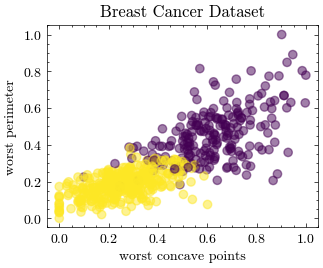
\includegraphics[width=\textwidth]{combined_files/combined_66_1.png}
    \end{center}
    { \hspace*{\fill} \\}
    
    \subsection{Activation Function}\label{activation-function}

Recall that the output of the perceptron was the dot product between the
weight vector \(\vec{w}\) and the input vector \(\vec{x}\) plus a
constant bias term \(b\)

Perceptron: \(y=w^Tx + b\)

Activation functions are applied after the computation.

    \subsubsection{Sigmoid Function}\label{sigmoid-function}

In order to do binary classification, we would like to limit the value
of the output to be in the range (0, 1) and get a value to represent the
probability of the output being assigned to either class. The sigmoid
function is perfect for this

\[ \sigma(z) = \frac{1}{1+e^-z} \]

\begin{tcolorbox}
\tiny
\begin{verbatim}
sigmoid = lambda x: 1 / (1 + np.exp(-x))
\end{verbatim}
\end{tcolorbox}

\begin{tcolorbox}
\tiny
\begin{verbatim}
def plot(fx, x_min, x_max, points=100, title=""):

    x = np.linspace(x_min, x_max, points)
    y = fx(x)

    fig, axes = plt.subplots()
    axes.plot(x, y)
    axes.set_xlabel("X")
    axes.set_ylabel("Y")
    axes.set_title("Activation Function")


x_min = -10
x_max = 10
points = 100
plot(sigmoid, x_min, x_max, points)
\end{verbatim}
\end{tcolorbox}

    \begin{center}
    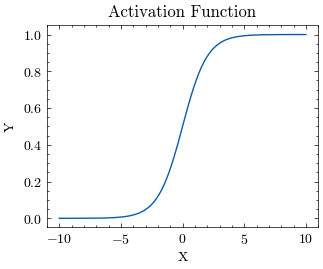
\includegraphics[width=\textwidth]{combined_files/combined_70_0.png}
    \end{center}
    { \hspace*{\fill} \\}
    
    \subsection{Gradient of Sigmoid
Function}\label{gradient-of-sigmoid-function}

Gradient Descent will be used later to find the optimal weight values.
As a result, let's calculate the gradient of the sigmoid function.

    \begin{align*}
\sigma^\prime
&= \frac{\partial}{\partial z} \sigma(z) \\
&= \frac{\partial}{\partial z} (\frac{1}{1+e^{-z}}) \\
&= \frac{\partial}{\partial z} (1+e^{-z})^{-1}) \\
&= (-1)(1+e^{-z})^{-2}\frac{\partial}{\partial z}(1+e^{-z}) \\
&= (-1)(1+e^{-z})^{-2}(e^{-z})\frac{\partial}{\partial z}(-z) \\
&= (-1)(1+e^{-z})^{-2}(e^{-z})(-1) \\
&= \frac{e^{-z}}{(1+e^{-z})^{2}}
\end{align*}

\begin{tcolorbox}
\tiny
\begin{verbatim}
sigmoid_prime = lambda x: np.exp(-x) / np.power((1 + np.exp(-x)), 2)
plot(sigmoid_prime, x_min, x_max, points)
\end{verbatim}
\end{tcolorbox}

    \begin{center}
    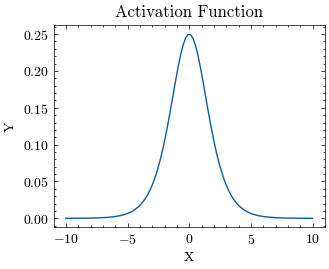
\includegraphics[width=\textwidth]{combined_files/combined_73_0.png}
    \end{center}
    { \hspace*{\fill} \\}
    
    \subsection{Autograd}\label{autograd}

Alternatively, you can use autograd to differentiate a numpy function.
Pytorch and JAX also implement autograd.

\begin{tcolorbox}
\tiny
\begin{verbatim}
# grad() differentiates scalar inputs
sigmoid_prime_grad = grad(sigmoid)
# egrad() differentiates vectorized inputs
sigmoid_prime_egrad = egrad(sigmoid)

x = np.linspace(x_min, x_max, points)
assert sigmoid_prime_grad(x[0]) == sigmoid_prime(x[0])
assert np.allclose(sigmoid_prime_egrad(x), sigmoid_prime(x))

plot(sigmoid_prime_egrad, x_min, x_max, points)
\end{verbatim}
\end{tcolorbox}

    \begin{center}
    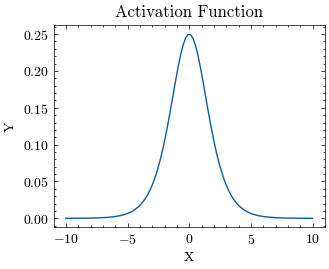
\includegraphics[width=\textwidth]{combined_files/combined_75_0.png}
    \end{center}
    { \hspace*{\fill} \\}
    
    \subsection{Loss Function}\label{loss-function}

The binary cross entropy loss function will be used for logistic
regression. This loss function is derived from the definition of maximum
likelihood estimation.

For the binary classification model, the probability of seeing the first
class is the sigmoid activation function is applied over the sum of the
bias \(b\) and the dot product of the weight vector \(\vec{w}\) and the
input vector \(\vec{x}\). The probability of seeing the other class is
the difference between 1 and the probability of seeing the other class.

\[ P(Y=1 \mid \vec{x}; \vec{w}, b) = \sigma{(\vec{w} \cdot \vec{x} + b)}
\]

\[ P(Y=0 \mid \vec{x}; \vec{w}, b) = 1 - P(Y=1 \mid \vec{x}; \vec{w}, b)
\]

    \subsubsection{Maximum Likelihood
Estimation}\label{maximum-likelihood-estimation}

Maximum likelihhod estimation finds the optimal weights and bias to
maximize the probability of seeing the training data.

The probability of getting the correct binary prediction function in
terms of \(\vec{w}\) and \(b\) is the following. This can also be
thought of as a Bernoulli distribution.

\[
P(Y \mid \vec{x}; \vec{w}, b) =
\left[ \sigma(\vec{w} \cdot \vec{x} + b) \right]^{y} \,
\left[ 1 - \sigma(\vec{w} \cdot \vec{x} + b) \right]^{1 - y}
\]

With a training dataset of \(i\) examples of \(\vec{x_i}\) features and
\(y_i\) labels, so the total probability is written as the product of
the probabilites of all the training examples. Consider this as the
likelihood of the training dataset with the current weights and bias.

\[
P(Y \mid \vec{x_i}; \vec{w}, b) 
= \prod_{i=1}^{n}
\left[ \sigma(\vec{w} \cdot \vec{x_i} + b) \right]^{y_i}
\left[ 1 - \sigma(\vec{w} \cdot \vec{x_i} + b) \right]^{1 - y_i}
\]

Keep in mind that we want to find the set of optimal parameters
\(\vec{w}\) and \(b\) that maximize the total likelihood.

\[
P(Y \mid \vec{x_i}; \vec{w}, b) 
= \max_{\vec{w}, b} \;
\prod_{i=1}^{n}
\left[ \sigma(\vec{w} \cdot \vec{x_i} + b) \right]^{y_i}
\left[ 1 - \sigma(\vec{w} \cdot \vec{x_i} + b) \right]^{1 - y_i}
\]

    In order to find the optimal weights and bias for the logistic
regression model, we use gradient descent, which is a solution to
optimization problems. We have to take the partial derivative of the
likelihood with respect to \(\vec{w}\) and \(b\).

In it's current form, the total probability is a lot of multiplications.
Per the product rule for derivatives, the partial derivatives will also
be a lot of multiplication. In order to avoid this, we can take the
logarithm of the likelihood, which converts the multiplications into
additions.

\begin{align*}
\ln(P(Y \mid \vec{x_i}; \vec{w}, b)) &= \max_{\vec{w}, b} \ln(\prod_{i=1}^{n} [\sigma{(\vec{w} \cdot \vec{x_i} + b)}]^{y_i} [1 - \sigma{(\vec{w} \cdot \vec{x_i} + b)}]^{1-y_i}) \\
&= \max_{\vec{w}, b} \sum_{i=1}^{n}[ \ln([\sigma{(\vec{w} \cdot \vec{x_i} + b)}]^{y_i} [1 - \sigma{(\vec{w} \cdot \vec{x_i} + b)}]^{1-y_i})] \\
&= \max_{\vec{w}, b} \sum_{i=1}^{n}[ \ln([\sigma{(\vec{w} \cdot \vec{x_i} + b)}]^{y_i}) + \ln([1 - \sigma{(\vec{w} \cdot \vec{x_i} + b)}]^{1-y_i})] \\
&= \max_{\vec{w}, b} \sum_{i=1}^{n}[ y_i \ln(\sigma{(\vec{w} \cdot \vec{x_i} + b)}) + (1-y_i) \ln(1 - \sigma{(\vec{w} \cdot \vec{x_i} + b)})] \\
\end{align*}

We define the negative (multiply equation above by -1) log of the
likelihood as the binary cross entropy loss function. Let's also divide
by the number of training examples to make this the average loss across
the \(n\) examples.

\begin{align*}
L(\vec{w}, b) = -\frac{1}{n}  \sum_{i=1}^{n}[ y_i \ln(\sigma{(\vec{w} \cdot \vec{x_i} + b)}) + (1-y_i) \ln(1 - \sigma{(\vec{w} \cdot \vec{x_i} + b)})] 
\end{align*}

    \subsubsection{Binary Cross Entropy Loss
Function}\label{binary-cross-entropy-loss-function}

Recall that
\(\hat y = \sigma{(\vec{w} \cdot \vec{x} + b)} = \frac{1}{1+e^-(\vec{w} \cdot \vec{x} + b)}\)

To simplify the calculation of the loss, let's rewrite it in terms of
\(\hat y\)

\begin{align*}
L(\hat y) &= -\frac{1}{n} \sum_{i=1}^{n} [y_i \ln(\hat y_i) + (1-y_i) \ln(1 - \hat y_i)]
\end{align*}

\begin{tcolorbox}
\tiny
\begin{verbatim}
def bce(y_true, y_pred):
    return -np.sum(y_true * np.log(y_pred) + (1 - y_true) * np.log(1 - y_pred))
\end{verbatim}
\end{tcolorbox}

    \subsection{Loss Function in Terms of W and
B}\label{loss-function-in-terms-of-w-and-b}

Before taking the partial derivative of the loss function with respect
to \(\vec{w}\) and \(b\). Let's simplify it to make the partial
derivative calculaton easier.

\(\hat y = \sigma{(\vec{w} \cdot \vec{x} + b)} = \frac{1}{1+e^-(\vec{w} \cdot \vec{x} + b)}\)

\begin{align*}
L(\vec{w}, b) &= -\frac{1}{n}  \sum_{i=1}^{n}[ y_i \ln(\sigma{(\vec{w} \cdot \vec{x_i} + b)}) + (1-y_i) \ln(1 - \sigma{(\vec{w} \cdot \vec{x_i} + b)})] \\ 
&= -\frac{1}{n}  \sum_{i=1}^{n}[ y_i \ln(\sigma{(\vec{w} \cdot \vec{x_i} + b)}) - y_i \ln(1 - \sigma{(\vec{w} \cdot \vec{x_i} + b)}) + \ln(1 - \sigma{(\vec{w} \cdot \vec{x_i} + b)})] \\ 
&= -\frac{1}{n}  \sum_{i=1}^{n}[ y_i \ln(\frac{\sigma{(\vec{w} \cdot \vec{x_i} + b)}}{1 - \sigma{(\vec{w} \cdot \vec{x_i} + b)}}) + \ln(1 - \sigma{(\vec{w} \cdot \vec{x_i} + b)})] \\
&= -\frac{1}{n}  \sum_{i=1}^{n}[ y_i \ln(\frac{\frac{1}{1+e^{-(\vec{w} \cdot \vec{x} + b)}}}{1 - \frac{1}{1+e^{-(\vec{w} \cdot \vec{x} + b)}}}) + \ln(1 - \frac{1}{1+e^{-(\vec{w} \cdot \vec{x} + b)}})] \\
&= -\frac{1}{n} \sum_{i=1}^{n} [y_i \ln(e^{\vec{w} \cdot \vec{x_i} + b}) + \ln(\frac{1}{1+e^{\vec{w} \cdot \vec{x_i} + b}})] \\ 
&= -\frac{1}{n} \sum_{i=1}^{n} [y_i (\vec{w} \cdot \vec{x_i} + b) - \ln(1+e^{\vec{w} \cdot \vec{x_i} + b})] \\ 
\end{align*}

    \subsection{Loss Function Gradient}\label{loss-function-gradient}

    Loss function with respect to \(W\)

\begin{align*}
\nabla_{W} [L(\vec{w}, b)] &= \nabla_{W} [-\frac{1}{n} \sum_{i=1}^{n} [y_i (\vec{w} \cdot \vec{x_i} + b) - \ln(1+e^{\vec{w} \cdot \vec{x_i} + b})]] \\
&= -\frac{1}{n} \sum_{i=1}^{n} [y_i \nabla_{W} [\vec{w} \cdot \vec{x_i} + b] - \nabla_{W}[\ln(1+e^{\vec{w} \cdot \vec{x_i} + b})]] \\
&= -\frac{1}{n} \sum_{i=1}^{n} [y_i x_i - (\frac{1}{1+e^{\vec{w} \cdot \vec{x_i} + b}}) \nabla_{W}[1+e^{\vec{w} \cdot \vec{x_i} + b}]] \\
&= -\frac{1}{n} \sum_{i=1}^{n} [y_i x_i - (\frac{1}{1+e^{\vec{w} \cdot \vec{x_i} + b}}) (e^{\vec{w} \cdot \vec{x_i} + b})\nabla_{W}[\vec{w} \cdot \vec{x_i} + b]] \\
&= -\frac{1}{n} \sum_{i=1}^{n} [y_i x_i - (\frac{1}{1+e^{\vec{w} \cdot \vec{x_i} + b}}) (e^{\vec{w} \cdot \vec{x_i} + b})(x_i)] \\
&= -\frac{1}{n} \sum_{i=1}^{n} [y_i x_i - x_i(\frac{e^{\vec{w} \cdot \vec{x_i} + b}}{1+e^{\vec{w} \cdot \vec{x_i} + b}})] \\
&= -\frac{1}{n} \sum_{i=1}^{n} [y_i x_i - x_i(\frac{1}{1+e^{-(\vec{w} \cdot \vec{x_i} + b)}})] \\ 
&= -\frac{1}{n} \sum_{i=1}^{n} [y_i x_i - x_i\hat y_i] \\ 
&= \frac{1}{n} \sum_{i=1}^{n} [\hat y_i x_i - y_i x_i  ] \\ 
&= \frac{1}{n} \sum_{i=1}^{n} [x_i (\hat y_i - y_i)] \\
\end{align*}

\begin{tcolorbox}
\tiny
\begin{verbatim}
def bce_dw(x, y_true, y_pred):
    return np.mean(x * (y_pred - y_true))
\end{verbatim}
\end{tcolorbox}

    Loss function with respect to \(b\)

\begin{align*}
\frac{\partial}{\partial b}  [L(\vec{w}, b)] &= \frac{\partial}{\partial b} [-\frac{1}{n} \sum_{i=1}^{n} [y_i (\vec{w} \cdot \vec{x_i} + b) - \ln(1+e^{\vec{w} \cdot \vec{x_i} + b})]] \\
&= -\frac{1}{n} \sum_{i=1}^{n} [y_i \frac{\partial}{\partial b} [\vec{w} \cdot \vec{x_i} + b] - \frac{\partial}{\partial b}[\ln(1+e^{\vec{w} \cdot \vec{x_i} + b})]] \\
&= -\frac{1}{n} \sum_{i=1}^{n} [y_i (1) - (\frac{1}{1+e^{\vec{w} \cdot \vec{x_i} + b}}) \frac{\partial}{\partial b}[1+e^{\vec{w} \cdot \vec{x_i} + b}] ] \\
&= -\frac{1}{n} \sum_{i=1}^{n} [y_i - (\frac{1}{1+e^{\vec{w} \cdot \vec{x_i} + b}}) (e^{\vec{w} \cdot \vec{x_i} + b}) \frac{\partial}{\partial b}[\vec{w} \cdot \vec{x_i} + b]] \\
&= -\frac{1}{n} \sum_{i=1}^{n} [y_i - (\frac{1}{1+e^{\vec{w} \cdot \vec{x_i} + b}}) (e^{\vec{w} \cdot \vec{x_i} + b}) (1)] \\
&= -\frac{1}{n} \sum_{i=1}^{n} [y_i - (\frac{e^{\vec{w} \cdot \vec{x_i} + b}}{1+e^{\vec{w} \cdot \vec{x_i} + b}})] \\
&= -\frac{1}{n} \sum_{i=1}^{n} [y_i - (\frac{1}{1+e^-({\vec{w} \cdot \vec{x_i} + b})})] \\
&= -\frac{1}{n} \sum_{i=1}^{n} [y_i - \hat y_i] \\
&= \frac{1}{n} \sum_{i=1}^{n} (\hat y_i - y_i) \\
\end{align*}

\begin{tcolorbox}
\tiny
\begin{verbatim}
def bce_db(y_true, y_pred):
    return np.mean(y_pred - y_true)
\end{verbatim}
\end{tcolorbox}

    \subsection{Gradient Descent}\label{gradient-descent}

With the binary cross entropy functions with respect to \(\vec{w}\) and
\(b\), the gradient descent equations are:

    Gradient Descent for weights \(\vec{w}\)

\begin{align*}
\vec{w} &= \vec{w} - \eta \nabla_{W} [L(\vec{w}, b)] \\
&= \vec{w} - \eta [\frac{1}{n} \sum_{i=1}^{n} [x_i (\hat y_i - y_i)]]
\end{align*}

    Gradient Descent for bias \(b\)

\begin{align*}
b &= b - \eta \frac{\partial}{\partial b} [L(\vec{w}, b)] \\
&= b - \eta [\frac{1}{n} \sum_{i=1}^{n} (\hat y_i - y_i)]
\end{align*}

\begin{tcolorbox}
\tiny
\begin{verbatim}
def gradient_descent(weights, x, bias, y_true, y_pred, learning_rate):
    weights = weights - learning_rate * bce_dw(x, y_true, y_pred)
    bias = bias - learning_rate * bce_db(y_true, y_pred)

    return weights, bias
\end{verbatim}
\end{tcolorbox}

    \subsection{Graphing functions}\label{graphing-functions}

Utility functions to create the visualizations

\begin{tcolorbox}
\tiny
\begin{verbatim}
def create_plots():
    fig, ax = plt.subplots(1, 3, figsize=(16 / 9.0 * 4, 4 * 1))
    fig.suptitle("Logistic Regression")

    ax[0].set_xlabel("Epoch", fontweight="normal")
    ax[0].set_ylabel("Error", fontweight="normal")
    ax[0].set_title("Binary Cross Entropy Error")

    ax[1].axis("off")
    ax[2].axis("off")

    ax[2] = fig.add_subplot(1, 2, 2, projection="3d")
    ax[2].set_xlabel("X")
    ax[2].set_ylabel("Y")
    ax[2].set_zlabel("Z")
    ax[2].set_title("Prediction Probabilities")
    ax[2].view_init(20, -35)

    camera = Camera(fig)
    return ax[0], ax[2], camera


def plot_graphs(
    ax0,
    ax1,
    idx,
    visible_mse,
    mse_idx,
    errors,
    features,
    labels,
    predictions,
    points_x,
    points_y,
    surface_predictions,
):
    ax0.plot(
        mse_idx[visible_mse][: idx + 1],
        errors[visible_mse][: idx + 1],
        color="red",
        alpha=0.5,
    )

    # Plot Logistic Regression Predictions
    # Ground truth and training data
    ground_truth_legend = ax1.scatter(
        features[:, 0],
        features[:, 1],
        labels,
        color="red",
        alpha=0.5,
        label="Ground Truth",
    )
    # Logistic Regression Predictions
    predictions_legend = ax1.scatter(
        features[:, 0],
        features[:, 1],
        predictions,
        color="blue",
        alpha=0.2,
        label="Prediction",
    )
    ax1.plot_surface(
        points_x,
        points_y,
        surface_predictions.reshape(dims, dims),
        color="blue",
        alpha=0.2,
    )
    ax1.legend(
        (ground_truth_legend, predictions_legend),
        ("Ground Truth", "Predictions"),
        loc="upper left",
    )
\end{verbatim}
\end{tcolorbox}

    \subsection{Training the model}\label{training-the-model}

\begin{tcolorbox}
\tiny
\begin{verbatim}
def fit(
    w0, b0, features, labels, dims, epochs, learning_rate, optimizer, output_filename
):
    mse_idx = np.arange(1, epochs + 1)
    errors = np.full(epochs, -1)
    ax0, ax1, camera = create_plots()

    points = np.linspace(0, 1, dims)
    points_x, points_y = np.meshgrid(points, points)
    surface_points = np.column_stack((points_x.flatten(), points_y.flatten()))

    weights = w0
    bias = b0

    for idx in range(epochs):
        error = 0
        predictions = np.array([])
        surface_predictions = np.array([])

        # fit the model on the training data
        for x, y in zip(features, labels):
            output = sigmoid(np.dot(weights, x) + bias)

            predictions = np.append(predictions, output)

            # Store Error
            error += bce(y, output)

            # Gradient Descent
            weights, bias = optimizer(weights, x, bias, y, output, learning_rate)

        # error /= len(features)

        # Visualization
        if (
            idx < 5
            or (idx < 15 and idx % 5 == 0)
            or (idx <= 50 and idx % 25 == 0)
            or (idx <= 1000 and idx % 200 == 0)
            or idx % 500 == 0
        ):
            for surface_point in surface_points:
                output = sigmoid(np.dot(weights, surface_point) + bias)
                surface_predictions = np.append(surface_predictions, output)

            print(f"epoch: {idx:>4}, BCA: {round(error, 2)}")

            # Plot BCE
            errors[idx] = error
            visible_mse = errors != -1

            plot_graphs(
                ax0,
                ax1,
                idx,
                visible_mse,
                mse_idx,
                errors,
                features,
                labels,
                predictions,
                points_x,
                points_y,
                surface_predictions,
            )

            camera.snap()

    animation = camera.animate()
    animation.save(output_filename, writer="pillow")
\end{verbatim}
\end{tcolorbox}

\begin{tcolorbox}
\tiny
\begin{verbatim}
epochs = 5001
learning_rate = 0.0005
dims = 10

w0 = np.random.rand(X[0].shape[0])
b0 = np.random.rand()

output_filename = "logistic_regression.gif"
fit(w0, b0, X, Y, dims, epochs, learning_rate, gradient_descent, output_filename)
\end{verbatim}
\end{tcolorbox}

    \begin{center}
    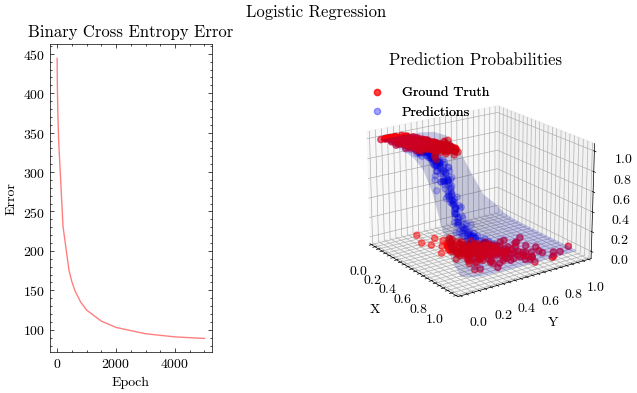
\includegraphics[width=\textwidth]{combined_files/combined_95_1.png}
    \end{center}
    { \hspace*{\fill} \\}
        
    \section{Perceptron}\label{perceptron}

The perceptron algorithm finds the optimal weights for a hyperplane to
separate two classes, which is also known as binary classification.

    Import the libraries

\begin{tcolorbox}
\tiny
\begin{verbatim}
import numpy as np

# %matplotlib ipympl
import matplotlib.pyplot as plt
from mpl_toolkits.mplot3d import Axes3D

from celluloid import Camera
import scienceplots
from IPython.display import Image

np.random.seed(0)
plt.style.use(["science", "no-latex"])
\end{verbatim}
\end{tcolorbox}

    \subsection{Training Dataset}\label{training-dataset}

Let's generate a dataset where the label is determined by a linear
decision boundary. Our perceptron will layer find the weights of a
normal vector to separate the dataset into two classes.

\begin{tcolorbox}
\tiny
\begin{verbatim}
def generate_dataset(dims, normal_vector):
    # create 3D grid of points
    points = np.linspace(-1, 1, dims)
    X, Y, Z = np.meshgrid(points, points, points)

    # features are the x, y, z coordinates
    features = np.column_stack((X.ravel(), Y.ravel(), Z.ravel()))

    # labels are the side each point is on the hyperplane
    distances = np.dot(features, normal_vector)
    labels = np.where(distances >= 0, 1, -1)
    return X, Y, Z, features, labels

# normalized normal vector
target_normal_vector = np.array([1.0, 1.0, 1.0])
target_normal_vector = target_normal_vector / np.linalg.norm(target_normal_vector)

scaling = 5
X, Y, Z, features, labels = generate_dataset(scaling, target_normal_vector)

fig = plt.figure()
ax = fig.add_subplot(111, projection="3d")

# plot the points
ax.scatter(features[:,0], features[:,1], features[:,2], marker='o', alpha=0.3, c=labels)
\end{verbatim}
\end{tcolorbox}
        
    \begin{center}
    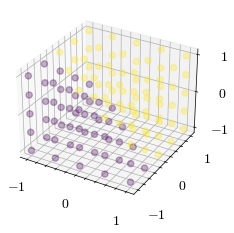
\includegraphics[width=\textwidth]{combined_files/combined_101_1.png}
    \end{center}
    { \hspace*{\fill} \\}
    
    \subsection{Hyperplane}\label{hyperplane}

A hyperplane is a flat subspace that is one less dimension than the
current space. It can be used to linearly separate a dataset. The
equation of a hyperplane is defined by the vector normal to the
hyperplane \(\vec{w}\)

\begin{align*}
\vec{w} \cdot \vec{x} = w_1 x_1 + ... + w_n x_n = 0
\end{align*}

In our case, the \(\vec{x}\) is the x, y, z coordinate.

\begin{align*}
\vec{w} \cdot \vec{x} &= 0 \\
&= w_1 x + w_2 y + w_3 z
\end{align*}

Since we want to perform binary classification using the side a point is
on relative from the hyperplane, the z value can be our predicted label

\begin{align*}
z = -(w_1 x + w_2 y) / w_3
\end{align*}

\begin{tcolorbox}
\tiny
\begin{verbatim}
def generate_hyperplane(scaling, normal_vector):
    # create 2D points
    points = np.linspace(-1, 1, scaling)
    xx, yy = np.meshgrid(points, points)

    # the z value is the defined by the hyperplane
    zz = -(normal_vector[0] * xx + normal_vector[1] * yy) / normal_vector[2]
    return xx, yy, zz

xx, yy, zz = generate_hyperplane(scaling, target_normal_vector)

# visualize the hyperplane
fig = plt.figure()
ax = fig.add_subplot(111, projection="3d")

# plot the hyperplane defined by the normal vector
ax.plot_surface(xx, yy, zz, alpha=0.2, color="gray")
ax.quiver(
    0,
    0,
    0,
    target_normal_vector[0],
    target_normal_vector[1],
    target_normal_vector[2],
    color="green",
    length=1,
    arrow_length_ratio=0.2,
)

ax.set_xlabel("X")
ax.set_ylabel("Y")
ax.set_zlabel("Z")
ax.set_title("Hyperplane")
\end{verbatim}
\end{tcolorbox}

            \begin{tcolorbox}[breakable, size=fbox, boxrule=.5pt, pad at break*=1mm, opacityfill=0]
\prompt{Out}{outcolor}{3}{\boxspacing}
\begin{Verbatim}[commandchars=\\\{\}]
Text(0.5, 0.92, 'Hyperplane')
\end{Verbatim}
\end{tcolorbox}
        
    \begin{center}
    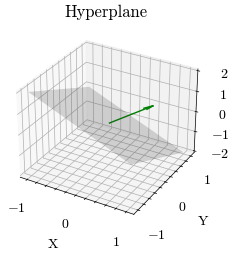
\includegraphics[width=\textwidth]{combined_files/combined_103_1.png}
    \end{center}
    { \hspace*{\fill} \\}
    
    \subsection{Loss Function: Hinge Loss}\label{loss-function-hinge-loss}

Loss functions are used to quantify the error of a prediction.

The perceptron uses the hinge loss function, which returns 0 for correct
predictions and 1 for incorrect predictions.

\begin{align*}
L(\vec{w}, b) = max(0, -y(\vec{w} \cdot \vec{x} + b)
\end{align*}

\begin{tcolorbox}
\tiny
\begin{verbatim}
def hinge_loss(w, x, b, y):
    return max(0.0, -y * (np.dot(w, x) + b))
\end{verbatim}
\end{tcolorbox}

    \subsection{Hinge Loss Gradient}\label{hinge-loss-gradient}

In order to run gradient descent to update our parameters, the gradients
with respect to W and b must be calculated

    \subsection{Hinge Loss Gradient in Terms of
B}\label{hinge-loss-gradient-in-terms-of-b}

Loss function with respect to \(b\)

\[
\frac{\partial L}{\partial b} =
\begin{cases}
0, & -y (\vec{w} \cdot \vec{x} + b) > 1 \\
-y, & \text{otherwise}
\end{cases}
\]

\begin{tcolorbox}
\tiny
\begin{verbatim}
def hinge_loss_db(w, x, b, y):
    if y * (np.dot(w, x) + b) <= 0.0:
        return -y
    return 0
\end{verbatim}
\end{tcolorbox}

    \subsection{Hinge Loss Gradient in Terms of
W}\label{hinge-loss-gradient-in-terms-of-w}

Loss function with respect to \(\vec{w}\)

\[
\nabla\{W\} {[}L(\vec{w}, b){]} =
\begin{cases}
0, & -y (\vec{w} \cdot \vec{x} + b) > 1 \\
-y \vec{x}, & \text{otherwise}
\end{cases}
\]

\begin{tcolorbox}
\tiny
\begin{verbatim}
def hinge_loss_dw(w, x, b, y):
    if y * (np.dot(w, x) + b) <= 0.0:
        return -y * x
    return np.zeros_like(x)
\end{verbatim}
\end{tcolorbox}

    \subsection{Graphing functions}\label{graphing-functions}

Utility functions to create the visualizations

\begin{tcolorbox}
\tiny
\begin{verbatim}
def create_plots():
    fig, ax = plt.subplots(2, 3, figsize=(16 / 9.0 * 4, 4 * 1), layout="constrained")
    fig.suptitle("Perceptron")

    ax[0, 0].set_xlabel("Epoch", fontweight="normal")
    ax[0, 0].set_ylabel("Error", fontweight="normal")
    ax[0, 0].set_title("Hinge Loss")

    ax[1, 0].set_xlabel("Z, Distance to Hyperplane", fontweight="normal")
    ax[1, 0].set_ylabel("", fontweight="normal")
    ax[1, 0].set_title("Linear Transformation")

    ax[0, 1].axis("off")
    ax[0, 2].axis("off")
    ax[1, 1].axis("off")
    ax[1, 2].axis("off")

    ax[1, 2] = fig.add_subplot(1, 2, 2, projection="3d")
    ax[1, 2].set_xlabel("X")
    ax[1, 2].set_ylabel("Y")
    ax[1, 2].set_zlabel("Z")
    ax[1, 2].set_title("Hyperplane Decision Boundary")
    ax[1, 2].view_init(20, -35)
    ax[1, 2].set_xlim(-1, 1)
    ax[1, 2].set_ylim(-1, 1)
    ax[1, 2].set_zlim(-1, 1)

    camera = Camera(fig)
    return ax[0, 0], ax[1, 0], ax[1, 2], camera


def plot_graphs(
    ax0,
    ax1,
    ax2,
    idx,
    visible_err,
    err_idx,
    errors,
    scaling,
    target_normal_vector,
    predictions,
    features,
    labels,
    weights,
):
    ax0.plot(
        err_idx[visible_err][: idx + 1],
        errors[visible_err][: idx + 1],
        color="red",
    )

    # Ground truth
    xx_target, yy_target, zz_target = generate_hyperplane(scaling, target_normal_vector)
    ground_truth_legend = ax2.plot_surface(
        xx_target,
        yy_target,
        zz_target,
        color="red",
        alpha=0.2,
        label="Ground Truth",
    )
    ax2.quiver(
        0,
        0,
        0,
        target_normal_vector[0],
        target_normal_vector[1],
        target_normal_vector[2],
        color="red",
        length=1,
        arrow_length_ratio=0.1,
    )

    # Perceptron predictions using 2D graph to show linear transformation
    def generate_colors(arr):
        return ["green" if d >= 0 else "orange" for d in arr]

    ground_truth_colors = generate_colors(labels)
    ax1.scatter(
        predictions,
        np.zeros(predictions.shape),
        c=ground_truth_colors,
        marker="o",
        alpha=0.3,
    )

    # Perceptron predictions using 3D graph to show hyperplane
    predictions_colors = generate_colors(predictions)
    predictions_norm = np.maximum(1 - np.exp(-(predictions**2)), 0.2)

    ax2.scatter(
        features[:, 0],
        features[:, 1],
        features[:, 2],
        c=predictions_colors,
        marker="o",
        alpha=predictions_norm,
    )

    xx, yy, zz = generate_hyperplane(scaling, weights)
    predictions_legend = ax2.plot_surface(
        xx,
        yy,
        zz,
        color="blue",
        alpha=0.2,
        label="Prediction",
    )
    ax2.quiver(
        0,
        0,
        0,
        weights[0],
        weights[1],
        weights[2],
        color="blue",
        length=1,
        arrow_length_ratio=0.1,
    )

    # Legend
    ax2.legend(
        (ground_truth_legend, predictions_legend),
        ("Ground Truth", "Predictions"),
        loc="upper left",
    )
\end{verbatim}
\end{tcolorbox}

    \subsection{Gradient Descent}\label{gradient-descent}

Gradient Descent will be used to update the weights and bias.

    Bias Gradient Descent:

\begin{align*}
b &= b - \eta \frac{\partial}{\partial b} [L(\vec{w}, b)] \\
&= b - \eta \begin{cases}
0 & -y(\vec{w} \cdot \vec{x} + b) > 1 \\
-y & \text{otherwise}
\end{cases}
\end{align*}

    Weights Gradient Descent:

\begin{align*}
\vec{w} &= \vec{w} - \eta \nabla_{W} [L(\vec{w}, b)] \\
&= \vec{w} - \eta \begin{cases}
0 & -y(\vec{w} \cdot \vec{x} + b) > 1 \\
-y x & \text{otherwise}
\end{cases}
\end{align*}

\begin{tcolorbox}
\tiny
\begin{verbatim}
def gradient_descent(weights, x, bias, y, learning_rate):
    weights = weights - learning_rate * hinge_loss_dw(weights, x, bias, y)
    bias = bias - learning_rate * hinge_loss_db(weights, x, bias, y)

    return weights, bias
\end{verbatim}
\end{tcolorbox}

    \subsection{Training the Model}\label{training-the-model}

\begin{tcolorbox}
\tiny
\begin{verbatim}
def fit(
    weights,
    bias,
    target_normal_vector,
    features,
    labels,
    X,
    Y,
    Z,
    scaling,
    epochs,
    learning_rate,
    optimizer,
    output_filename,
):
    err_idx = np.arange(1, epochs + 1)
    errors = np.full(epochs, -1)
    ax0, ax1, ax2, camera = create_plots()

    for idx in range(epochs):
        error = 0
        predictions = np.array([])

        for x, y in zip(features, labels):
            # Forward Propagation
            output = np.dot(weights, x) + bias

            predictions = np.append(predictions, output)

            # Store Error
            error += hinge_loss(weights, x, bias, y)

            # Gradient Descent
            weights, bias = optimizer(weights, x, bias, y, learning_rate)

        error /= len(X)
        weights = weights / np.linalg.norm(weights)

        if (
            idx < 5
            or (idx < 15 and idx % 2 == 0)
            or (idx <= 50 and idx % 10 == 0)
            or (idx <= 1000 and idx % 20 == 0)
            or idx % 250 == 0
        ):

            print(f"epoch: {idx}, MSE: {error}")

            # Plot MSE
            errors[idx] = error
            visible_err = errors != -1

            plot_graphs(
                ax0,
                ax1,
                ax2,
                idx,
                visible_err,
                err_idx,
                errors,
                scaling,
                target_normal_vector,
                predictions,
                features,
                labels,
                weights,
            )

            camera.snap()

    animation = camera.animate()
    animation.save(output_filename, writer="pillow")
    plt.show()
\end{verbatim}
\end{tcolorbox}

    Let's put everything together and train our Perceptron

\begin{tcolorbox}
\tiny
\begin{verbatim}
weights = np.array([1.0, -1.0, -1.0])
weights = weights / np.linalg.norm(weights)

bias = 0
\end{verbatim}
\end{tcolorbox}

\begin{tcolorbox}
\tiny
\begin{verbatim}
epochs = 301
learning_rate = 0.0005

output_filename = "perceptron.gif"
fit(
    weights,
    bias,
    target_normal_vector,
    features,
    labels,
    X,
    Y,
    Z,
    scaling,
    epochs,
    learning_rate,
    gradient_descent,
    output_filename,
)
\end{verbatim}
\end{tcolorbox}

    \begin{center}
    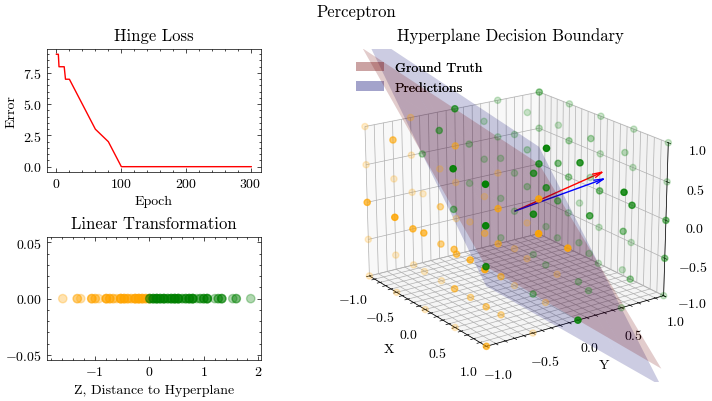
\includegraphics[width=\textwidth]{combined_files/combined_121_1.png}
    \end{center}
    { \hspace*{\fill} \\}
        
    \section{Neural Network Weights
Visualization}\label{neural-network-weights-visualization}

Neural Networks at a high-level just consist of matrix multiplications
at each layer. Matrix multiplications are linear transformations. This
visualization shows the linear transformations at each layer and the
loss landscape of each layer. This Notebook builds on top of the
\texttt{Neural\ Network} Notebook. Look at the previous Notebook for the
derivation of Backpropagation and the math behind neural networks.

    Gavin's Note: The goal of this visualization is show that
Backpropagation updates the weights and biases in the most optimal way.
In order to visualize this, this program changes the weights to make
them non optimal to show that the loss increases. As a result, this
program will take a very long time.

\begin{tcolorbox}
\tiny
\begin{verbatim}
import numpy as np
import torch
import torch.nn as nn
import torch.nn.functional as F

# %matplotlib ipympl
import matplotlib.pyplot as plt
from mpl_toolkits.mplot3d import Axes3D

from celluloid import Camera
import scienceplots
from IPython.display import Image

torch.manual_seed(0)
np.random.seed(0)
plt.style.use(["science", "no-latex"])
\end{verbatim}
\end{tcolorbox}

    \subsection{Training Dataset}\label{training-dataset}

Let's generate a non-linear dataset, since neural networks can fit this
function while linear models, such as a perceptron, can't converge on
this dataset

\begin{tcolorbox}
\tiny
\begin{verbatim}
# generate the non-linear dataset, meaning that a hyperplane can't separate the data
def generate_XOR():
    N = 500
    X = np.random.rand(N, 2)
    y = (X[:, 0] > 0.5) != (X[:, 1] > 0.5)

    return X, y


X, y = generate_XOR()

fig = plt.figure()
ax = fig.add_subplot()
ax.scatter(X[:, 0], X[:, 1], c=y, alpha=0.5)
\end{verbatim}
\end{tcolorbox}
        
    \begin{center}
    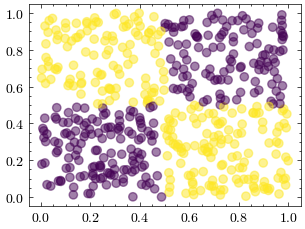
\includegraphics[width=\textwidth]{combined_files/combined_128_1.png}
    \end{center}
    { \hspace*{\fill} \\}
    
    \subsection{Graph Functions}\label{graph-functions}

In our training function, we use the gradient descent optimizer to
update the weights and move on. What if we didn't use the weights from
the optimizer? These graphing functions manually change the values in
the weight matrix of our neural network's layers and run the neural
network to see how the loss changes.

There are also graphing functions that show the linear transformation of
each layer.

\begin{tcolorbox}
\tiny
\begin{verbatim}
def create_scatterplots(rows=2, cols=3, width_scale=1, height_scale=1):
    fig, axes = plt.subplots(
        rows,
        cols,
        figsize=(16 / 9.0 * 4 * width_scale, 4 * height_scale),
        layout="constrained",
    )
    axes = axes.flatten()

    layer_idx = 0
    for i, axis in enumerate(axes):
        if not ((i + 1) % cols == 0):
            axis.set_title(f"Layer {layer_idx}")
            layer_idx += 1

    axes[-1].set_title("Predictions")
    axes[-1 - cols].set_title("Mean Squared Error")

    camera = Camera(fig)
    return axes, camera


def create_3d_plots(rows=2, cols=3, width_scale=1, height_scale=1):
    fig = plt.figure(
        figsize=(16 / 9.0 * 4 * width_scale, 4 * height_scale), layout="constrained"
    )
    axes = []

    layer_idx = 0
    for i in range(rows * cols):
        if not ((i + 1) % cols == 0):
            axis = fig.add_subplot(rows, cols, i + 1, projection="3d")
            axis.set_title(f"Layer {layer_idx + 1}")
            axes.append(axis)
            layer_idx += 1
        else:
            axes.append(fig.add_subplot(rows, cols, i + 1))

    axes[-1].set_title("Predictions")
    axes[-1 - cols].set_title("Mean Squared Error")

    camera = Camera(fig)
    return axes, camera


def plot_layer_loss_landscape(
    axis,
    model,
    target_layer_idx,
    neuron_idx,
    features,
    labels,
    w1_min,
    w1_max,
    w2_min,
    w2_max,
    loss_dims,
    device,
    color="blue",
):
    """Plot how the loss changes when the first two weights in the first neuron change"""
    loss_fn = nn.MSELoss()

    init = model.get_values(target_layer_idx, neuron_idx)
    w1 = init[0].item()
    w2 = init[1].item()

    target_layer_idx = target_layer_idx % len(model.layers)

    w1_range = torch.linspace(w1_min + w1, w1_max + w1, loss_dims).to(device)
    w2_range = torch.linspace(w2_min + w2, w2_max + w2, loss_dims).to(device)
    w1_range, w2_range = torch.meshgrid(w1_range, w2_range, indexing="ij")
    w_range = torch.stack((w1_range.flatten(), w2_range.flatten()), axis=1)

    error_range = np.array([])

    for target_layer_weight in w_range:
        model.override_layer_weight(
            target_layer_idx, neuron_idx, init + target_layer_weight
        )
        error = 0
        for x, y in zip(features, labels):
            output = model(x)
            y = y.unsqueeze(0)
            loss = loss_fn(output, y)
            error += loss.detach().cpu().numpy()
        error /= len(labels)
        error_range = np.append(error_range, error)

        if np.isclose(target_layer_weight[0].item(), w1, atol=0.25) and np.isclose(
            target_layer_weight[1].item(), w2, atol=0.25
        ):
            axis.scatter([w1], [w2], [error], color=color, alpha=0.4)

    axis.plot_surface(
        w1_range.detach().cpu().numpy(),
        w2_range.detach().cpu().numpy(),
        error_range.reshape(loss_dims, loss_dims),
        color=color,
        alpha=0.1,
    )
    model.override_layer_weight(target_layer_idx, neuron_idx, init)


def plot_mse_and_predictions(
    axes, features, idx, visible_mse, mse_idx, errors, predictions, cmap, cols, device
):
    features_cpu = features.detach().cpu().numpy()

    # Plot MSE
    mse_ax = axes[-1 - cols]
    mse_ax.plot(
        mse_idx[visible_mse][: idx + 1],
        errors[visible_mse][: idx + 1],
        color="red",
        alpha=0.5,
    )
    mse_ax.plot(
        [1],
        [0],
        color="white",
        alpha=0,
    )

    # Plot Predictions
    predictions_classes = np.where(predictions > 0.5, 1, 0)

    predictions_ax = axes[-1]
    predictions_ax.scatter(
        features_cpu[:, 0],
        features_cpu[:, 1],
        c=predictions_classes,
        cmap=cmap,
        alpha=0.5,
    )


def plot_transformations_and_predictions(
    axes,
    model,
    idx,
    visible_mse,
    mse_idx,
    errors,
    predictions,
    features,
    labels,
    cmap,
    rows,
    cols,
    device,
):
    plot_mse_and_predictions(
        axes,
        features,
        idx,
        visible_mse,
        mse_idx,
        errors,
        predictions,
        cmap,
        cols,
        device,
    )
    model.visualize(features, labels, axes, cmap, rows, cols)


def plot_loss_landscape_and_predictions(
    axes,
    model,
    idx,
    visible_mse,
    mse_idx,
    errors,
    predictions,
    features,
    labels,
    cmap,
    cols,
    device,
    w1_min=-5,
    w1_max=5,
    w2_min=-5,
    w2_max=5,
    loss_dims=7,
):
    # this uses axes with index -1 and -1-cols
    plot_mse_and_predictions(
        axes,
        features,
        idx,
        visible_mse,
        mse_idx,
        errors,
        predictions,
        cmap,
        cols,
        device,
    )

    num_layers = len(model.layers)

    target_layer_idx = -1

    for index, axis in enumerate(reversed(axes)):
        # in reverse order, predictions plot is index 0 and mse plot is index cols
        if index == 0 or index == cols or abs(target_layer_idx) > num_layers:
            continue
        plot_layer_loss_landscape(
            axis,
            model,
            target_layer_idx,
            0,
            features,
            labels,
            w1_min,
            w1_max,
            w2_min,
            w2_max,
            loss_dims,
            device,
            color="blue",
        )
        if target_layer_idx != -1:
            plot_layer_loss_landscape(
                axis,
                model,
                target_layer_idx,
                1,
                features,
                labels,
                w1_min,
                w1_max,
                w2_min,
                w2_max,
                loss_dims,
                device,
                color="red",
            )
        target_layer_idx -= 1
\end{verbatim}
\end{tcolorbox}

    \subsection{PyTorch Implementation}\label{pytorch-implementation}

Let's define a feedforward neural network in PyTorch, but add custom
functions to each layer that manually change the weight values. We want
to use this function to see how the loss changes when the weights aren't
at the optimal value. This is used to show that Backpropagation tells us
how to update the weights optimally.

\begin{tcolorbox}
\tiny
\begin{verbatim}
class VisualNet(nn.Module):
    def __init__(self):
        super(VisualNet, self).__init__()
        self.layers = nn.ModuleList()

    def visualize(self, X, y, axes, cmap, rows, cols):
        y_cpu = y.detach().cpu().numpy()

        layer_idx = 0
        for i, axis in enumerate(axes):
            if not ((i + 1) % cols == 0):
                X_cpu = X.detach().cpu().numpy()

                # input and hidden layer outputs
                if X.shape[1] != 1:
                    axis.scatter(
                        X_cpu[:, 0], X_cpu[:, 1], c=y_cpu, cmap=cmap, alpha=0.5
                    )
                # output layer is 1D, so set second dimenstional to zeros
                else:
                    axis.scatter(
                        X_cpu[:, 0],
                        np.zeros(X_cpu[:, 0].shape),
                        c=y_cpu,
                        cmap=cmap,
                        alpha=0.5,
                    )

                if layer_idx < len(self.layers):
                    X = F.tanh(self.layers[layer_idx](X))
                    layer_idx += 1

    def override_layer_weight(self, layer_idx, neuron_idx, new_weights):
        if (abs(layer_idx) > len(self.layers)) or (
            abs(neuron_idx) > len(self.layers[layer_idx].weight)
        ):
            return

        with torch.no_grad():
            self.layers[layer_idx].weight[neuron_idx, :2] = new_weights

    def get_values(self, layer_idx, neuron_idx):
        if (abs(layer_idx) > len(self.layers)) or (
            abs(neuron_idx) > len(self.layers[layer_idx].weight)
        ):
            return torch.zeros(2)

        with torch.no_grad():
            return self.layers[layer_idx].weight.detach().clone()[neuron_idx, :2]


class TorchNet(VisualNet):
    def __init__(self, num_hidden_layers):
        super().__init__()

        # define the layers
        self.input_layer = nn.Linear(2, 2)
        self.layers.append(self.input_layer)

        for i in range(num_hidden_layers):
            self.layers.append(nn.Linear(2, 2))

        self.output_layer = nn.Linear(2, 1)
        self.layers.append(self.output_layer)

    def forward(self, x):
        # pass the result of the previous layer to the next layer
        for layer in self.layers[:-1]:
            x = F.tanh(layer(x))

        return self.output_layer(x)
\end{verbatim}
\end{tcolorbox}

    \subsection{Training the Model}\label{training-the-model}

Similar to the previous Neural Network Notebook, let's pass in the
training data to our model, update the weights with our optimizer, and
update our visualization

\begin{tcolorbox}
\tiny
\begin{verbatim}
def torch_fit(
    model,
    features,
    labels,
    epochs,
    learning_rate,
    transformations_plot_filename,
    loss_landscape_plot_filename,
    device,
    rows=2,
    cols=3,
    width_scale=1,
    height_scale=1,
):
    mse_idx = np.arange(1, epochs + 1)
    errors = np.full(epochs, -1)

    cmap = plt.cm.colors.ListedColormap(["red", "blue"])

    scatterplots, camera1 = create_scatterplots(rows, cols, width_scale, height_scale)
    loss_plots, camera2 = create_3d_plots(rows, cols, width_scale, height_scale)

    loss_fn = nn.MSELoss()
    optimizer = torch.optim.SGD(model.parameters(), lr=learning_rate, momentum=0.3)

    for idx in range(epochs):
        error = 0
        predictions = np.array([])

        for x, y in zip(features, labels):
            # Forward Propagation
            output = model(x)

            output_np = output.detach().cpu().numpy()
            predictions = np.append(predictions, output_np)

            # Store Error
            # tensor(0.) -> tensor([0.]) to match shape of output variable
            y = y.unsqueeze(0)
            loss = loss_fn(output, y)

            error += loss.detach().cpu().numpy()

            # Backpropagation
            optimizer.zero_grad()
            loss.backward()
            optimizer.step()

        if (
            idx < 5
            or (idx <= 50 and idx % 5 == 0)
            or (idx <= 1000 and idx % 50 == 0)
            or idx % 250 == 0
        ):
            print(f"epoch: {idx}, MSE: {error}")

            # Plot MSE
            errors[idx] = error
            visible_mse = errors != -1

            plot_transformations_and_predictions(
                scatterplots,
                model,
                idx,
                visible_mse,
                mse_idx,
                errors,
                predictions,
                features,
                labels,
                cmap,
                rows,
                cols,
                device,
            )

            plot_loss_landscape_and_predictions(
                loss_plots,
                model,
                idx,
                visible_mse,
                mse_idx,
                errors,
                predictions,
                features,
                labels,
                cmap,
                cols,
                device,
            )

            camera1.snap()
            camera2.snap()

    animation1 = camera1.animate()
    animation1.save(transformations_plot_filename, writer="pillow")
    animation2 = camera2.animate()
    animation2.save(loss_landscape_plot_filename, writer="pillow")

    plt.show()
\end{verbatim}
\end{tcolorbox}

    \subsection{Visualize the transformations and weight
updates}\label{visualize-the-transformations-and-weight-updates}

Let's call our training function with our model to create the
visualization.

\begin{tcolorbox}
\tiny
\begin{verbatim}
device = torch.device("cuda:0" if torch.cuda.is_available() else "cpu")
torch_model = TorchNet(num_hidden_layers=2).to(device)

rows = 2
cols = 3

# the inputs and outputs for PyTorch must be tensors
X_tensor = torch.tensor(X, device=device, dtype=torch.float32).squeeze(-1)
y_tensor = torch.tensor(y, device=device, dtype=torch.float32).squeeze(-1)

epochs = 601
learning_rate = 0.005

transformations_plot_filename = "neural_network_weights.gif"
loss_landscape_plot_filename = "neural_network_weights_loss_landscape.gif"
torch_fit(
    torch_model,
    X_tensor,
    y_tensor,
    epochs,
    learning_rate,
    transformations_plot_filename,
    loss_landscape_plot_filename,
    device,
    rows=rows,
    cols=cols,
)
\end{verbatim}
\end{tcolorbox}

    \begin{center}
    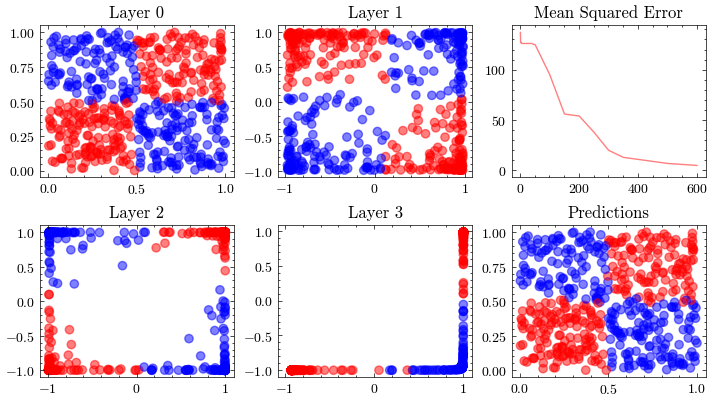
\includegraphics[width=\textwidth]{combined_files/combined_136_1.png}
    \end{center}
    { \hspace*{\fill} \\}
    
    \begin{center}
    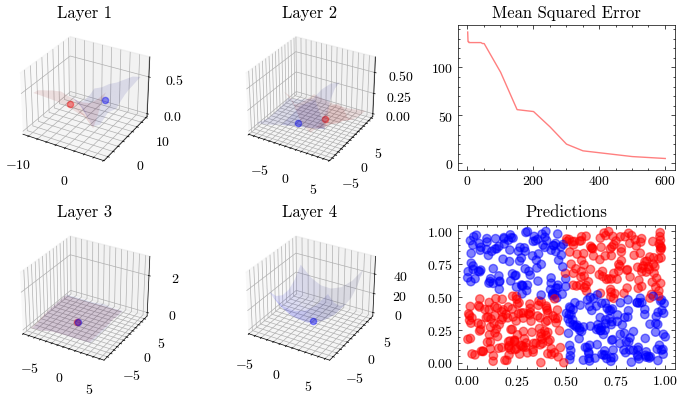
\includegraphics[width=\textwidth]{combined_files/combined_136_2.png}
    \end{center}
    { \hspace*{\fill} \\}
    
    This visualization shows the internal linear transformation of each
layer in the neural network. We will show each layer transform an input
to an output. At the 3rd layer, the data becomes linearly separable. As
a result of these transformations, the network is able to classify
inputs into these two classes.
        
    This visualization shows that the weights all update together such that
the loss function at the last layer reaches the minima. See how the 3D
plot in layer 4 is at a minima.
        
    \subsection{Vanishing Gradients}\label{vanishing-gradients}

It's a valid assumption that increasing the number of layers of a neural
network allows it to recognize more patterns. However, scaling is not
this straightforward. With the wrong architectures, the networks can
stop scaling. The next visualization increases the number of layers to
12 and shows that the weights can not update. This is known as vanishing
gradients since the updates being sent to the earlier layers in the
network are close to zero, preventing the weights from updating. The
ResNet paper introduced residual connections, which helped solved this
issue.

    \subsubsection{12 Layer Neural Network}\label{layer-neural-network}

Let's rerun our code but with a larger network this time

\begin{tcolorbox}
\tiny
\begin{verbatim}
device = torch.device("cuda:0" if torch.cuda.is_available() else "cpu")
torch_model = TorchNet(num_hidden_layers=10).to(device)

rows = 2
cols = 7

X_tensor = torch.tensor(X, device=device, dtype=torch.float32).squeeze(-1)
y_tensor = torch.tensor(y, device=device, dtype=torch.float32).squeeze(-1)

epochs = 1001
learning_rate = 0.005

width_scale = 4
height_scale = 2

transformations_plot_filename = "vanishing_gradients/layers_12.gif"
loss_landscape_plot_filename = "vanishing_gradients/layers_12_loss_landscape.gif"
torch_fit(
    torch_model,
    X_tensor,
    y_tensor,
    epochs,
    learning_rate,
    transformations_plot_filename,
    loss_landscape_plot_filename,
    device,
    rows=rows,
    cols=cols,
    width_scale=width_scale,
    height_scale=height_scale,
)
\end{verbatim}
\end{tcolorbox}

    \begin{center}
    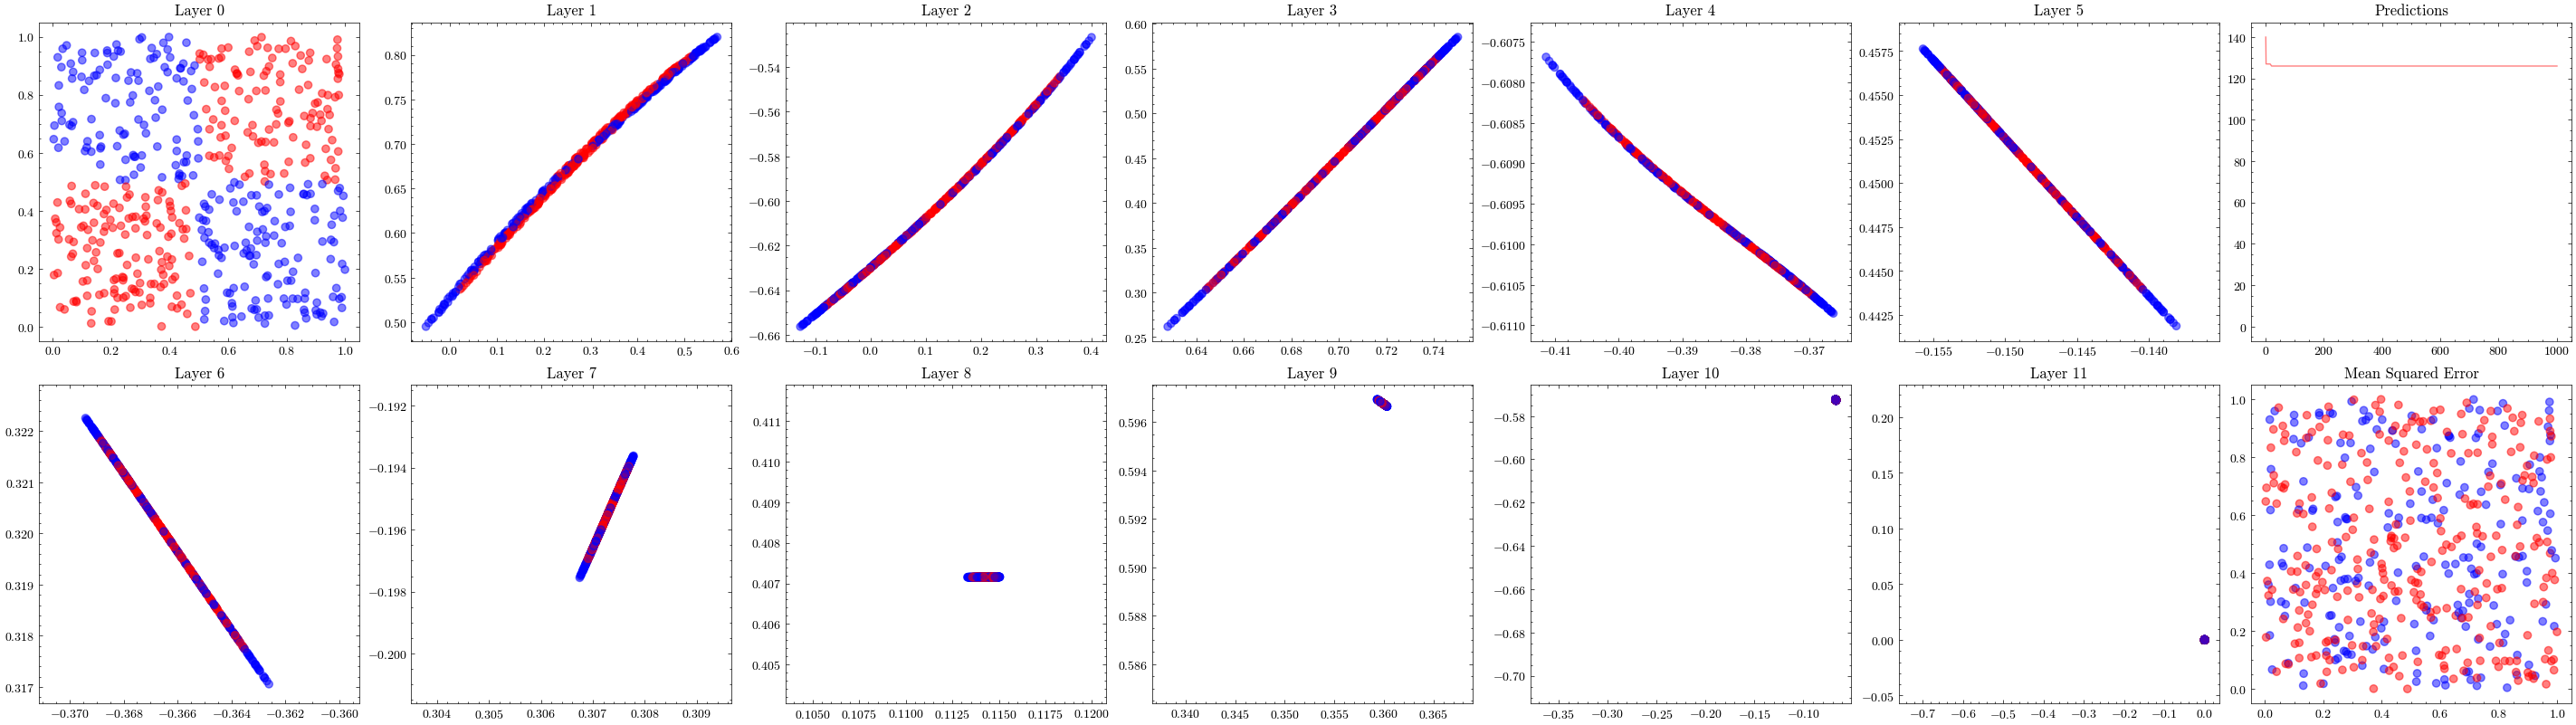
\includegraphics[width=\textwidth]{combined_files/combined_143_1.png}
    \end{center}
    { \hspace*{\fill} \\}
    
    \begin{center}
    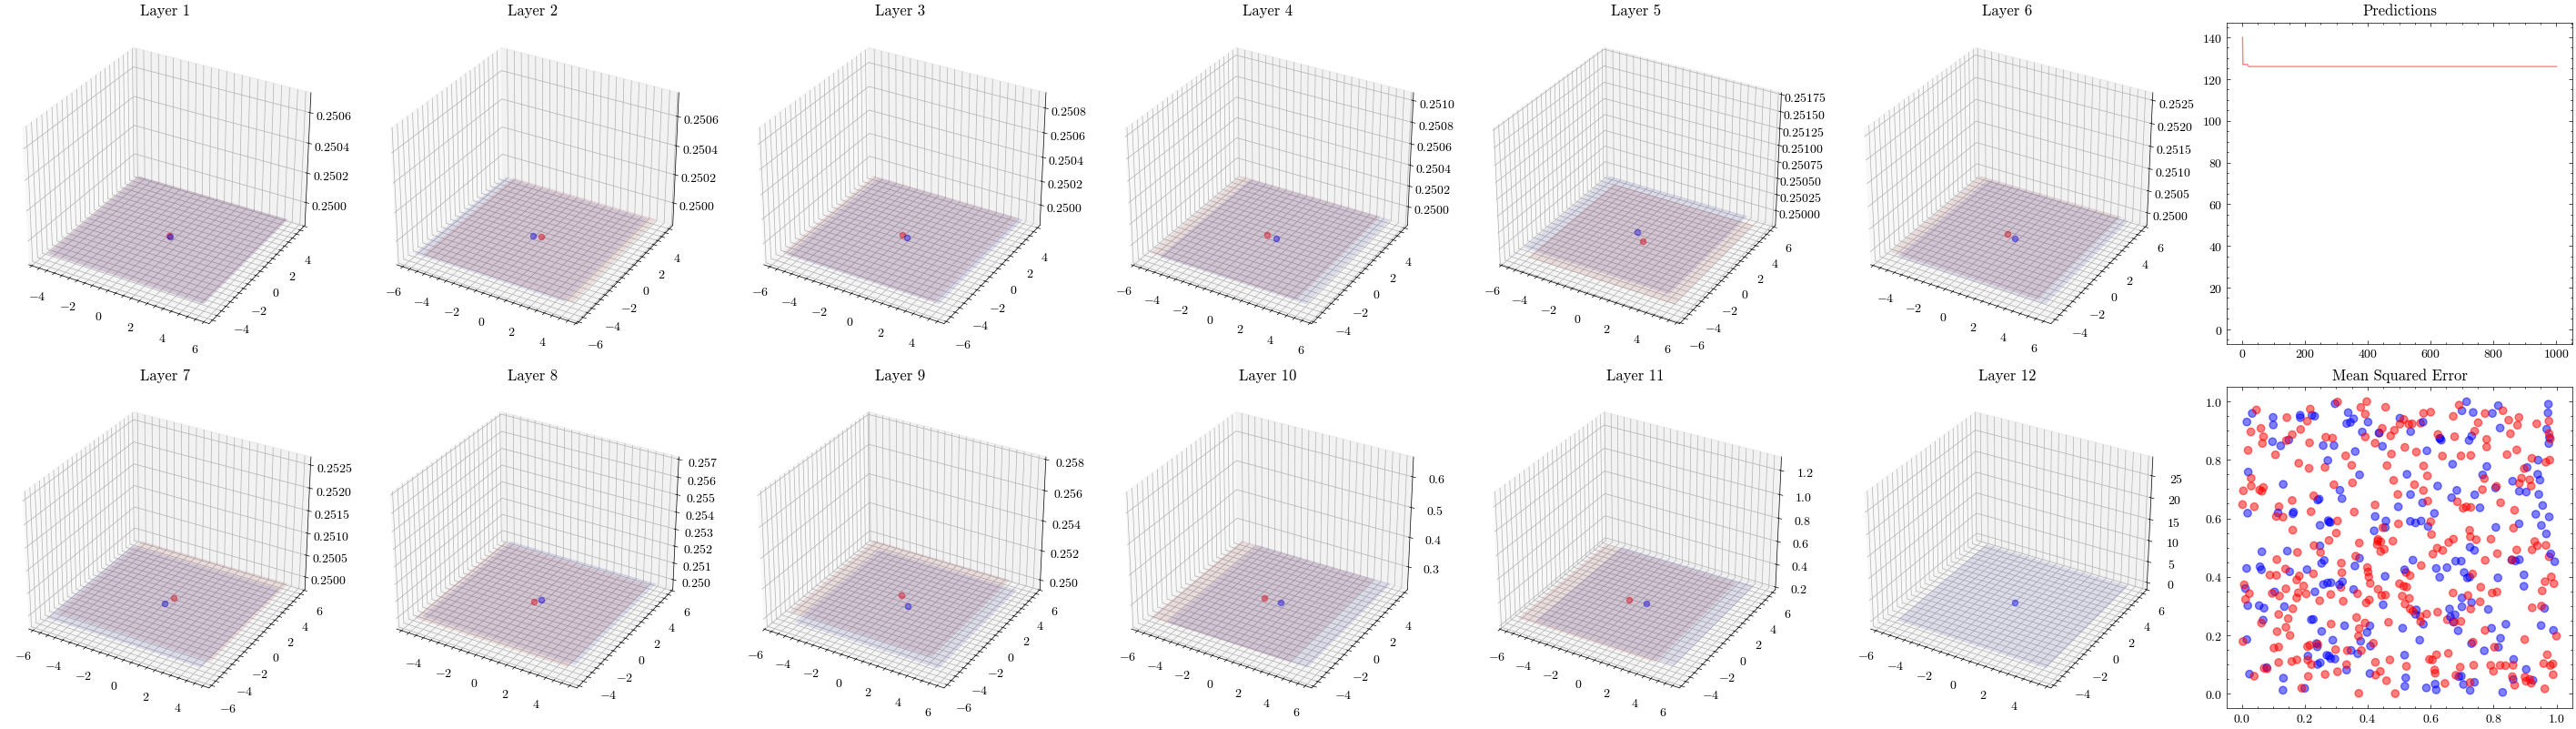
\includegraphics[width=\textwidth]{combined_files/combined_143_2.png}
    \end{center}
    { \hspace*{\fill} \\}
    
    In the visualizations below, we see the earlier layers not updating at
all from vanishing gradients.
        
    \section{Neural Network}\label{neural-network}

Neural Networks are a machine learning model that learns the optimal
parameters to approximate complex functions.

GitHub Repo: https://github.com/gavinkhung/neural-network

    Import the libraries

\begin{tcolorbox}
\tiny
\begin{verbatim}
import numpy as np

%matplotlib ipympl
import matplotlib.pyplot as plt
from mpl_toolkits.mplot3d import Axes3D

from celluloid import Camera
import scienceplots
from IPython.display import Image

np.random.seed(0)
plt.style.use(["science", "no-latex"])
\end{verbatim}
\end{tcolorbox}

    \subsection{Training Dataset}\label{training-dataset}

The neural network will learn the parameters to fit a Hyperbolic
Paraboloid.

\begin{align*}
z &= \frac{y^2}{b^2} - \frac{x^2}{a^2}
\end{align*}

\begin{tcolorbox}
\tiny
\begin{verbatim}
def generate_function(dims):
    a = 1
    b = 1

    # Hyperbolic Paraboloid
    x = np.linspace(-1, 1, dims)
    y = np.linspace(-1, 1, dims)
    X, Y = np.meshgrid(x, y)
    Z = (Y**2 / b**2) - (X**2 / a**2)

    X_t = X.flatten()
    Y_t = Y.flatten()
    Z_t = Z.flatten()
    X_t = X_t.reshape((len(X_t), 1))
    Y_t = Y_t.reshape((len(Y_t), 1))
    Z_t = Z_t.reshape((len(Z_t), 1))
    features = np.stack((X_t, Y_t), axis=1)
    labels = Z_t.reshape((len(Z_t), 1, 1))

    return X, Y, Z, features, labels


dims = 12
X, Y, Z, features, labels = generate_function(dims)

# Visualize the Hyperbolic Paraboloid
fig = plt.figure()
ax = fig.add_subplot(111, projection="3d")

ax.plot_surface(X, Y, Z, color="red", alpha=0.5)
\end{verbatim}
\end{tcolorbox}
        
    \begin{center}
    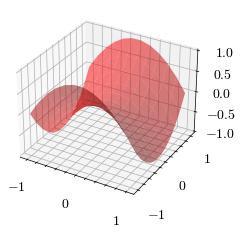
\includegraphics[width=\textwidth]{combined_files/combined_151_1.png}
    \end{center}
    { \hspace*{\fill} \\}
    
    \subsection{Loss Function}\label{loss-function}

The loss function is needed to evaluate the performance of the model and
to update the weights accordingly. The optimizaton process of the neural
network training will find the weights and biases to minimie the loss.

    \subsubsection{Mean Squared Error}\label{mean-squared-error}

Quadratic loss functions, like mean squared error, are used for
regression tasks, like this example.

\[
J = \frac{1}{n} \sum_{i=1}^{n} (y_i - \hat{y}_i)^2
\]

\begin{tcolorbox}
\tiny
\begin{verbatim}
def mse(y_true, y_pred):
    return np.mean(np.power(y_true - y_pred, 2))
\end{verbatim}
\end{tcolorbox}

    \subsubsection{Mean Squared Error
Gradient}\label{mean-squared-error-gradient}

In order to perform backpropagation to update the weights, we need to
calculate the gradient of the loss function.

\begin{align*}
J^{\prime} &= \frac{\partial}{\partial \hat{y}} [ \frac{1}{n} \sum_{i=1}^{n}(y_{i}-\hat{y})^2 ] \\
&= \frac{1}{n} \sum_{i=1}^{n}\frac{\partial}{\partial \hat{y}} [ (y_{i}-\hat{y})^2 ] \\
&= \frac{2}{n} \sum_{i=1}^{n} (y_{i}-\hat{y}) \frac{\partial}{\partial \hat{y}}[y_{i}-\hat{y}] \\
&= \frac{2}{n} \sum_{i=1}^{n} (y_{i}-\hat{y}) (-1) \\
&= \frac{2}{n} \sum_{i=1}^{n}(\hat{y}-y_{i})
\end{align*}

\begin{tcolorbox}
\tiny
\begin{verbatim}
def mse_prime(y_true, y_pred):
    return 2 * (y_pred - y_true) / np.size(y_true)
\end{verbatim}
\end{tcolorbox}

    \subsection{Neural Network Layer}\label{neural-network-layer}

We will implement a feedforward neural network, which contains many
layers. Each layer at a very high applies a linear transformation to the
input data to create the output data, which is often in a different
dimension than the input data. Then, all of the values in the output are
run through a function, known as an activation function.

Recall from Linear Algebra that an input column vector \(x\) in
\(\mathbb{R}^n\) can be transformed into another dimension
\(\mathbb{R}^m\) by multipying it with a matrix of size \(m \times n\).
Finally we can add a bias term to this linear transformation to shift
the transformed data up or down.

As a result, each layer stores a weight matrix and a bias vector to
apply the linear transformation.

\begin{tcolorbox}
\tiny
\begin{verbatim}
from abc import ABC, abstractmethod


class Layer(ABC):
    def __init__(self):
        self.input = None
        self.output = None
        self.weights = None
        self.bias = None

    @abstractmethod
    def forward(self, input):
        pass

    @abstractmethod
    def backward(self, output_gradient, optimizer):
        pass
\end{verbatim}
\end{tcolorbox}

    \subsection{Forward Propagation}\label{forward-propagation}

This the process of transforming our input data into the predictions
from our feedforward neural network. The input data is passed through
every layer of the network. 

    Each neuron in a layer is a weighted sum of its inputs plus a bias term.
Finally, an activation function is applied on each neuron in the layer.
We will have a class to represent a fully-connected layer and another
class to represent an activation function.

The computation for each neuron in a layer being a weighted sum of the
products between the inputs and the layer's weights plus a bias term is
the same as a matrix multiplication between the weight matrix and the
input data added with a bias vector.

Thus, the forward propagation of a fully connected layer can be written
as:

\begin{align*}
Z &= W X + B \\
A &= g(Z)
\end{align*}

Where: - \(W\) is the weight matrix for the layer - \(X\) is the input
data - \(B\) is a bias vector - \(g\) is the activation function

    \subsection{Our Network's Forward
Propagation}\label{our-networks-forward-propagation}

    We will implement a 3-layer fully-connected neural network with a Tanh
activation function after each layer. These transformations can be
written as these matrix multiplications:

\begin{align*}
Z_1 &= W_1 X + B_1 \\
A_1 &= tanh(Z_1) \\
\\
Z_2 &= W_2 A_1 + B_2 \\
A_2 &= tanh(Z_2) \\
\\
Z_3 &= W_3 A_2 + B_3 \\
\hat{y} &= A_3 = tanh(Z_3)
\end{align*}

    \subsection{Backpropagation}\label{backpropagation}

Backpropagation is the process of updating all of the weights and biases
in a neural network using the chain rule and gradient descent.

The following equations use \(J\) as our loss function. In this
Notebook, we use the mean squared error loss function. Click
\hyperref[mean-squared-error]{here for the mean squared error loss function}.

Our goal is to apply gradient descent on the weights and bias using the
following equations:

\begin{align*}
W_1 &= W_1 - lr * \frac{\partial J}{\partial W_1} \\
B_1 &= B_1 - lr * \frac{\partial J}{\partial B_1} \\
W_2 &= W_2 - lr * \frac{\partial J}{\partial W_2} \\
B_2 &= B_2 - lr * \frac{\partial J}{\partial B_2} \\
W_3 &= W_3 - lr * \frac{\partial J}{\partial W_3} \\
B_3 &= B_3 - lr * \frac{\partial J}{\partial B_3} \\
\end{align*}

We need to use the chain rule to get the values for
\(\frac{\partial J}{\partial W_1}\),
\(\frac{\partial J}{\partial B_1}\),
\(\frac{\partial J}{\partial W_2}\),
\(\frac{\partial J}{\partial B_2}\),
\(\frac{\partial J}{\partial W_3}\), and
\(\frac{\partial J}{\partial B_3}\).

    \subsubsection{Chain Rule for
Backpropagation}\label{chain-rule-for-backpropagation}

Let's derive a general formula to update the weight matrix \(W_i\) and
bias vector \(B_i\) of a single fully-connected layer.

To apply gradient descent on the 3rd layer, for example, we need to find
the loss with respect to \(W_3\) and \(B_3\), which are
\(\frac{\partial J}{\partial W_3}\), and
\(\frac{\partial J}{\partial B_3}\).

The loss function \(J\) is in terms of \(A_3\), which is the final
output/activation of the last layer. Then, \(A_3\) is in terms of
\(Z_3\). Lastly, \(Z_3\) is in terms of \(W_3\), \(B_3\), and \(A_2\),
which is the activation from the second to last layer. Let's get the
loss with respect to \(W_3\) and \(B_3\).

We can represent these matrix operations as the following composite
functions: \(J(A_3)\), \(A_3(Z_3)\), and \(Z_3(W_3, B_3, A_2)\)

Click
\hyperref[our-network-s-forward-propagation]{here for the operations of each layer}.

    \subsubsection{Chain Rule For Weight Matrix
W}\label{chain-rule-for-weight-matrix-w}

Use the chain rule to derive \(\frac{\partial J}{\partial W_3}\)

\begin{align*}
\frac{\partial J}{\partial W_3} &= \frac{\partial}{\partial W_3}[J(A_3(Z_3(W_3, B_3, A_2)))] \\
&= \frac{\partial J}{\partial A_3} \frac{\partial}{\partial W_3}[A_3(Z_3(W_3, B_3, A_2))] \\
&= \frac{\partial J}{\partial A_3} \frac{\partial A_3}{\partial Z_3} \frac{\partial}{\partial W_3}[Z_3(W_3, B_3, A_2))] \\
&= \frac{\partial J}{\partial A_3} \frac{\partial A_3}{\partial Z_3} \frac{\partial Z_3}{\partial W_3} \\
\end{align*}

    \subsubsection{Chain Rule For Bias Vector
B}\label{chain-rule-for-bias-vector-b}

Use the chain rule to derive \(\frac{\partial J}{\partial B_3}\).

\begin{align*}
\frac{\partial J}{\partial B_3} &= \frac{\partial}{\partial B_3}[J(A_3(Z_3(W_3, B_3, A_2)))] \\
&= \frac{\partial J}{\partial A_3} \frac{\partial}{\partial B_3}[A_3(Z_3(W_3, B_3, A_2))] \\
&= \frac{\partial J}{\partial A_3} \frac{\partial A_3}{\partial B_3} \frac{\partial}{\partial B_3}[Z_3(W_3, B_3, A_2))] \\
&= \frac{\partial J}{\partial A_3} \frac{\partial A_3}{\partial Z_3} \frac{\partial Z_3}{\partial B_3} \\
\end{align*}

    \subsection{Backpropagation for Weight Matrix
W}\label{backpropagation-for-weight-matrix-w}

\begin{align*}
\frac{\partial J}{\partial W_3} = \frac{\partial J}{\partial A_3} \frac{\partial A_3}{\partial Z_3} \frac{\partial Z_3}{\partial W_3}
\end{align*}

Let's break each component down:

\begin{enumerate}
\def\labelenumi{\arabic{enumi}.}
\item
  \(\frac{\partial J}{\partial A_3}\) is the gradient of the loss
  function, which is the gradient of the mean squared error function.
  Click
  \hyperref[mean-squared-error-gradient]{here for the derivation of the loss function gradient}.
  In the general case for any layer, this is the gradient from the next
  layer (idx+1).
\item
  \[\frac{\partial A_3}{\partial Z_3} =
  \frac{\partial}{\partial Z_3}{[}tanh(Z\_3){]} \] is the gradient of
  the activation function. Click
  \hyperref[tanh-activation-function-gradient]{here for the derivation of the activation function gradient}.
\item
  \(\frac{\partial Z_3}{\partial W_3} = \frac{\partial}{\partial W_3}[W_3 A_2 + B_3] = A_2\)
  is the original input to the layer, which is the output of the
  previous layer (idx-1).
\end{enumerate}

As a result, to the gradient of the weight matrix of a fully-connected
layer is the matrix multiplication products of the following: 1. The
gradient from the next layer (idx+1) 2. The gradient of the activation
function 3. The input from the previous layer (idx-1)

    \subsection{Backpropagation for Bias Vector
B}\label{backpropagation-for-bias-vector-b}

\begin{align*}
\frac{\partial J}{\partial B_3} = \frac{\partial J}{\partial A_3} \frac{\partial A_3}{\partial Z_3} \frac{\partial Z_3}{\partial B_3}
\end{align*}

Let's break each component down:

\begin{enumerate}
\def\labelenumi{\arabic{enumi}.}
\item
  \(\frac{\partial J}{\partial A_3}\) is the gradient of the loss
  function, which is the gradient of the mean squared error function.
  Click
  \hyperref[mean-squared-error-gradient]{here for the derivation of the loss function gradient}.
  In the general case for any layer, this is the gradient from the next
  layer (idx+1).
\item
  \(\frac{\partial A_3}{\partial Z_3}\) is the gradient of the
  activation function. Click
  \hyperref[tanh-activation-function-gradient]{here for the derivation of the activation function gradient}.
\item
  \(\frac{\partial Z_3}{\partial B_3} = \frac{\partial}{\partial B_3}[W_3 A_2 + B_3] = 1\)
  is 1, we can ignore this in the gradient computation.
\end{enumerate}

As a result, to the gradient of the bias vector of a fully-connected
layer is the matrix multiplication products of the following: 1. The
gradient from the next layer (idx+1) 2. The gradient of the activation
function

    For more information, I recommend the follow resources: -
\href{https://www.youtube.com/watch?v=pauPCy_s0Ok}{Neural Network from
Scratch}. I also watched this video to help write this Notebook. -
\href{https://www.youtube.com/watch?v=SmZmBKc7Lrs}{The Most Important
Algorithm in Machine Learning}

    \subsection{Dense Layers}\label{dense-layers}

A dense layer is a fully connected layer. Let's use the equations
derived in the forward and backwards propagation sections above to
implement the \texttt{forward()} and \texttt{backward()} methods of our
dense layer class.

\begin{tcolorbox}
\tiny
\begin{verbatim}
class Dense(Layer):
    def __init__(self, input_neurons, output_neurons):
        # Random Values from Normal Distribution
        # self.weights = np.random.randn(output_neurons, input_neurons)
        # self.bias = np.random.randn(output_neurons, 1)

        # All Zeros
        # self.weights = np.zeros((output_neurons, input_neurons))
        # self.bias = np.zeros((output_neurons, 1))

        # Xavier Initialization Uniform Distribution
        limit = np.sqrt(6 / (input_neurons + output_neurons))
        self.weights = np.random.uniform(
            -limit, limit, size=(output_neurons, input_neurons)
        )
        self.bias = np.zeros((output_neurons, 1))

    def forward(self, input):
        self.input = input
        return np.matmul(self.weights, self.input) + self.bias

    def backward(self, output_gradient, optimizer):
        # Calculate gradients
        weights_gradient = np.matmul(output_gradient, self.input.T)
        input_gradient = np.dot(self.weights.T, output_gradient)

        # Update weights and biases
        self.weights, self.bias = optimizer.backward(
            self.weights, weights_gradient, self.bias, output_gradient
        )
        return input_gradient
\end{verbatim}
\end{tcolorbox}

    \subsection{Activation Function}\label{activation-function}

Activation functions are applied after the matrix multiplication to
introduce nonlinearity into our neural networks. Choosing the correct
activation function is essential for the neural network to learn general
patterns of the training data. Most notably, the ReLU function is very
useful when training very deep neural networks with many layers, as seen
from the 2012 AlexNet paper, in order to prevent vanishing gradients,
where the network fails to update its weights from super small gradients

\begin{tcolorbox}
\tiny
\begin{verbatim}
class Activation(Layer):
    def __init__(self, activation, activation_prime):
        self.activation = activation
        self.activation_prime = activation_prime

    def forward(self, input_val):
        self.input = input_val
        return self.activation(self.input)

    def backward(self, output_gradient, optimizer):
        return np.multiply(output_gradient, self.activation_prime(self.input))

    def plot(self, x_min, x_max, points=25):
        x = np.linspace(x_min, x_max, points)
        y = self.activation(x)
        y_prime = self.activation_prime(y)

        fig, axes = plt.subplots(1, 2)
        axes[0].plot(x, y)
        axes[0].set_xlabel("X")
        axes[0].set_ylabel("Y")
        axes[0].set_title("F(X)")

        axes[1].plot(x, y_prime)
        axes[1].set_xlabel("X")
        axes[1].set_ylabel("Y")
        axes[1].set_title("F'(X)")
\end{verbatim}
\end{tcolorbox}

    \subsubsection{Tanh Activation Function}\label{tanh-activation-function}

We will use the Tanh activation function for our network:

\begin{align*}
\sigma(z) &= \frac{e^z-e^{-z}}{e^z+e^{-z}}
\end{align*}

    \subsubsection{Tanh Activation Function
Gradient}\label{tanh-activation-function-gradient}

Since gradient descent relies on knowing the gradient of our activation
function, let's derivate the gradient of the tanh function.

\begin{align*}
\sigma^\prime(z) &= \frac{\partial}{\partial z} [ \frac{e^z-e^{-z}}{e^z+e^{-z}} ] \\
&= \frac{(e^z+e^{-z})\frac{\partial}{\partial z}[e^z-e^{-z}] - (e^z-e^{-z})\frac{\partial}{\partial z}[e^z+e^{-z}]}{({e^z+e^{-z}})^2} \\
&= \frac{(e^z+e^{-z})(e^z+e^{-z}) - (e^z-e^{-z})(e^z-e^{-z})}{({e^z+e^{-z}})^2} \\
&= \frac{(e^z+e^{-z})^2 - (e^z-e^{-z})^2}{({e^z+e^{-z}})^2} \\
&= \frac{(e^z+e^{-z})^2}{({e^z+e^{-z}})^2} - \frac{(e^z-e^{-z})^2}{({e^z+e^{-z}})^2} \\
&= 1 - [\sigma(z)]^2
\end{align*}

    Now that we have derived the gradient of the Tanh function, let's create
the class for the Tanh activation function.

\begin{tcolorbox}
\tiny
\begin{verbatim}
class Tanh(Activation):
    def __init__(self):
        tanh = lambda x: np.tanh(x)
        tanh_prime = lambda x: 1 - np.tanh(x) ** 2
        super().__init__(tanh, tanh_prime)


Tanh().plot(-3, 3)
\end{verbatim}
\end{tcolorbox}

    \begin{center}
    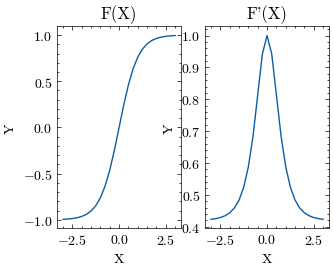
\includegraphics[width=\textwidth]{combined_files/combined_177_0.png}
    \end{center}
    { \hspace*{\fill} \\}
    
    \subsection{Optimizer}\label{optimizer}

Our optimization algorithm will be Gradient Descent, allowing us to
determine how to update the parameters in the next iteration.
$ X\_\{n+1\} = X\_n - lr * \frac{\partial}{\partial X} f(X\_n)$.

Let's create a class that updates the weight matrix and the bias vector
using the Gradient Descent equation.

\begin{tcolorbox}
\tiny
\begin{verbatim}
class GradientDescentOptimizier:
    def __init__(self, learning_rate):
        self.learning_rate = learning_rate

    def backward(self, weights, weights_gradient, bias, output_gradient):
        weights -= self.learning_rate * weights_gradient
        bias -= self.learning_rate * output_gradient

        return weights, bias
\end{verbatim}
\end{tcolorbox}

    \subsection{Graphing Functions}\label{graphing-functions}

This Notebook will create many visualizations of the neural network
during its training phase.

\texttt{create\_scatter\_and\_3d\_plot()} creates a 2 column graph for
the Mean Squared Error graph on the left and a 3D graph on the right.

\texttt{create\_3d\_and\_3d\_plot()} creates a 2 column graph with two
3D graphs.

\texttt{plot\_3d\_predictions()} plots the neural network's current
preditions and the expected output of the neural network.

\texttt{plot\_layer\_loss\_landscape()} plots how close one layer's
current weights are from the optimal weights by seeing how the total
mean squared error changes if the weights were shifted a little.

\begin{tcolorbox}
\tiny
\begin{verbatim}
import copy


def create_scatter_and_3d_plot():
    fig, ax = plt.subplots(1, 3, figsize=(16 / 9.0 * 4, 4 * 1))
    fig.suptitle("Neural Network Predictions")

    ax[0].set_xlabel("Epoch", fontweight="normal")
    ax[0].set_ylabel("Error", fontweight="normal")
    ax[0].set_title("Mean Squared Error")

    ax[1].axis("off")
    ax[2].axis("off")

    ax[2] = fig.add_subplot(1, 2, 2, projection="3d")
    ax[2].set_xlabel("X")
    ax[2].set_ylabel("Y")
    ax[2].set_zlabel("Z")
    ax[2].set_title("Function Approximation")
    ax[2].view_init(20, -35)
    ax[2].set_zlim(-1, 1)
    ax[2].axis("equal")

    camera = Camera(fig)
    return ax[0], ax[2], camera


def create_3d_and_3d_plot():
    fig, ax = plt.subplots(
        1, 2, figsize=(16 / 9.0 * 4, 4 * 1), subplot_kw={"projection": "3d"}
    )
    fig.suptitle("Neural Network Loss Landscape")

    ax[0].set_xlabel("W3_1")
    ax[0].set_ylabel("W3_2")
    ax[0].set_zlabel("MSE")
    ax[0].set_title("Mean Squared Error")
    ax[0].view_init(20, -35)
    ax[0].set_zlim(-1, 1)
    ax[0].axis("equal")

    ax[1].set_xlabel("X")
    ax[1].set_ylabel("Y")
    ax[1].set_zlabel("Z")
    ax[1].set_title("Function Approximation")
    ax[1].view_init(20, -35)
    ax[1].set_zlim(-1, 1)
    ax[1].axis("equal")

    camera = Camera(fig)
    return ax[0], ax[1], camera


def plot_3d_predictions(ax, X, Y, Z, predictions, dims):
    # Plot Neural Network Function Approximation
    # Ground truth
    ground_truth_legend = ax.plot_surface(
        X, Y, Z, color="red", alpha=0.5, label="Ground Truth"
    )

    # Neural Network Predictions
    predictions_legend = ax.scatter(
        X,
        Y,
        predictions.reshape((dims, dims)),
        color="blue",
        alpha=0.2,
        label="Prediction",
    )
    ax.plot_surface(
        X,
        Y,
        predictions.reshape((dims, dims)),
        color="blue",
        alpha=0.3,
    )
    ax.legend(
        (ground_truth_legend, predictions_legend),
        ("Ground Truth", "Predictions"),
        loc="upper left",
    )


def plot_layer_loss_landscape(
    ax0,
    network,
    target_layer_idx,
    features,
    labels,
    w1_min,
    w1_max,
    w2_min,
    w2_max,
    loss_dims,
):
    # current target layer weights
    target_layer_idx = target_layer_idx % len(network)

    w1 = network[target_layer_idx].weights[0][0]
    w2 = network[target_layer_idx].weights[0][1]
    curr_error = 0
    for x, y in zip(features, labels):
        output = x
        for layer in network:
            output = layer.forward(output)

        curr_error += mse(y, output)
    curr_error /= labels.size
    ax0.scatter([w1], [w2], [curr_error], color="red", alpha=0.4)

    target_layer = copy.deepcopy(network[target_layer_idx])
    w1_range = np.linspace(w1_min, w1_max, loss_dims)
    w2_range = np.linspace(w2_min, w2_max, loss_dims)
    w1_range, w2_range = np.meshgrid(w1_range, w2_range)
    w_range = np.stack((w1_range.flatten(), w2_range.flatten()), axis=1)

    error_range = np.array([])

    for target_layer_weight in w_range:
        target_layer_weight = target_layer_weight.reshape(1, 2)
        target_layer.weights[0, :2] = target_layer_weight[0, :2]

        error = 0
        for x, y in zip(features, labels):
            output = x
            for layer_idx, layer in enumerate(network):
                if layer_idx == target_layer_idx:
                    output = target_layer.forward(output)
                else:
                    output = layer.forward(output)

            error += mse(y, output)
        error /= labels.size
        error_range = np.append(error_range, error)

    ax0.plot_surface(
        w1_range,
        w2_range,
        error_range.reshape(loss_dims, loss_dims),
        color="blue",
        alpha=0.1,
    )


def plot_mse_and_predictions(
    ax0, ax1, idx, visible_mse, mse_idx, errors, X, Y, Z, predictions, dims
):
    ax0.plot(
        mse_idx[visible_mse][: idx + 1],
        errors[visible_mse][: idx + 1],
        color="red",
        alpha=0.5,
    )

    plot_3d_predictions(ax1, X, Y, Z, predictions, dims)


def plot_loss_landscape_and_predictions(
    ax0,
    ax1,
    network,
    target_layer_idx,
    features,
    labels,
    X,
    Y,
    Z,
    predictions,
    preds_dims,
    w1_min=-5,
    w1_max=5,
    w2_min=-5,
    w2_max=5,
    loss_dims=20,
):
    plot_3d_predictions(ax1, X, Y, Z, predictions, preds_dims)
    plot_layer_loss_landscape(
        ax0,
        network,
        target_layer_idx,
        features,
        labels,
        w1_min,
        w1_max,
        w2_min,
        w2_max,
        loss_dims,
    )


def show_epoch(epoch):
    return (
        epoch < 25
        or (epoch < 25 and epoch % 2 == 0)
        or (epoch <= 100 and epoch % 10 == 0)
        or (epoch <= 500 and epoch % 25 == 0)
        or (epoch <= 1000 and epoch % 50 == 0)
        or epoch % 250 == 0
    )
\end{verbatim}
\end{tcolorbox}

    \subsection{Training the model}\label{training-the-model}

Let's tie everything together to train the neural network. In each
epoch, we will do the following:

\begin{enumerate}
\def\labelenumi{\arabic{enumi}.}
\tightlist
\item
  Pass the training data into our model to get the model's predictions
\item
  Calculate the loss from the model's predictions and the expected value
\item
  Use the loss to run the optimizer to update the weights and biases
\item
  Call the visualization functions to visualize the training process
\end{enumerate}

\begin{tcolorbox}
\tiny
\begin{verbatim}
def fit(
    network,
    features,
    labels,
    X,
    Y,
    Z,
    preds_dims,
    epochs,
    optimizer,
    mse_plot_filename,
    loss_landscape_plot_filename,
):
    mse_idx = np.arange(1, epochs + 1)
    errors = np.full(epochs, -1)
    mse_ax, predictions_ax1, camera1 = create_scatter_and_3d_plot()
    loss_landscape_ax, predictions_ax2, camera2 = create_3d_and_3d_plot()

    network_len = len(network)

    for idx in range(epochs):
        error = 0
        predictions = np.array([])

        for x, y in zip(features, labels):
            # Forward Propagation
            output = x
            for layer in network:
                output = layer.forward(output)

            predictions = np.append(predictions, output)

            # Store Error
            # no need to convert to numpy cpu, since both are tensors on device
            error += mse(y, output)

            # Backpropagation
            grad = mse_prime(y, output)
            for layer in reversed(network):
                grad = layer.backward(grad, optimizer)

        error /= len(X)

        if show_epoch(idx):
            print(f"epoch: {idx}, MSE: {error}")

            # Plot MSE
            errors[idx] = error
            visible_mse = errors != -1
            plot_mse_and_predictions(
                mse_ax,
                predictions_ax1,
                idx,
                visible_mse,
                mse_idx,
                errors,
                X,
                Y,
                Z,
                predictions,
                preds_dims,
            )

            # plot the loss landscape of the second to last layer
            # a 3D plot can be made because it's only 2 neurons
            plot_loss_landscape_and_predictions(
                loss_landscape_ax,
                predictions_ax2,
                network,
                -2,
                features,
                labels,
                X,
                Y,
                Z,
                predictions,
                preds_dims,
            )

            camera1.snap()
            camera2.snap()

    animation1 = camera1.animate()
    animation1.save(mse_plot_filename, writer="pillow")

    animation2 = camera2.animate()
    animation2.save(loss_landscape_plot_filename, writer="pillow")
    plt.show()
\end{verbatim}
\end{tcolorbox}

    The model can be visualized with the following:

    Our model consists of 3 layers with the Tanh() activation function after
each layer.

Layer 1: - Input Dimensions: 2 - Output Dimensions: 12

Layer 2: - Input Dimensions: 12 - Output Dimensions: 2

Layer 3: - Input Dimensions: 2 - Output Dimensions: 1

\begin{tcolorbox}
\tiny
\begin{verbatim}
model = [Dense(2, 12), Tanh(), Dense(12, 2), Tanh(), Dense(2, 1), Tanh()]
\end{verbatim}
\end{tcolorbox}

    Let's train our model by passing our model and optimizer to our training
method

\begin{tcolorbox}
\tiny
\begin{verbatim}
epochs = 301
learning_rate = 0.005
optimizer = GradientDescentOptimizier(learning_rate)

mse_plot_filename = "neural_network.gif"
loss_landscape_plot_filename = "neural_network_loss_landscape.gif"
fit(
    model,
    features,
    labels,
    X,
    Y,
    Z,
    dims,
    epochs,
    optimizer,
    mse_plot_filename,
    loss_landscape_plot_filename,
)
\end{verbatim}
\end{tcolorbox}

    \begin{center}
    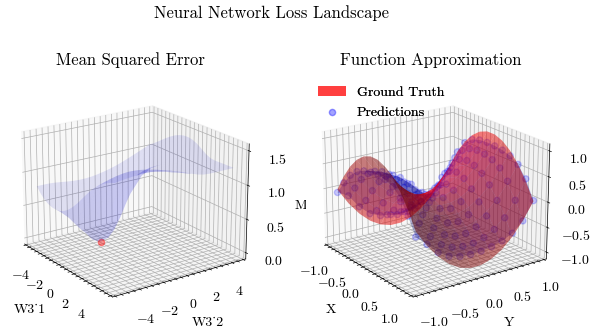
\includegraphics[width=\textwidth]{combined_files/combined_188_1.png}
    \end{center}
    { \hspace*{\fill} \\}
    
    \begin{center}
    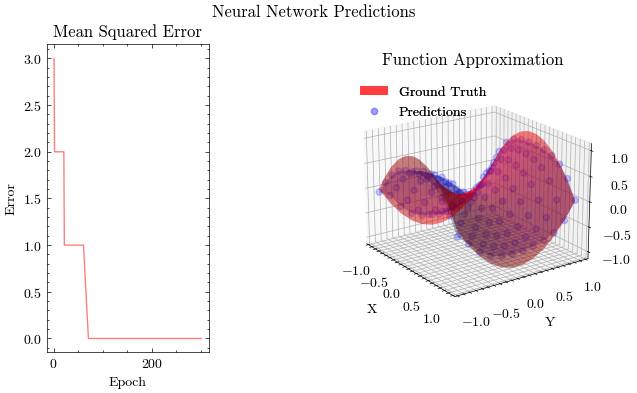
\includegraphics[width=\textwidth]{combined_files/combined_188_2.png}
    \end{center}
    { \hspace*{\fill} \\}
    
    \subsection{Output GIF}\label{output-gif}

In this visualization, we see the predictions fit the ground truth. The
neural network was able to find the optimal parameters to fit this
function. Now think about the applications of this. Given input data
about people's shopping habits, we can predict things to recommend to
them. We can recommend a social media post to show them or a show to
watch next. We can pass data to neural networks and it will uncover
patterns from input data and find patterns.
        
    The visualization below shows that backpropagation finds the optimal
weights for the neural network. On the left graph, the red dot shows the
current values of the weight matrix in the last layer of the neural
network. The z axis is the mean squared error loss. If the weights
weren't at the current value, the loss wouldn't be at a minima, meaning
that backpropagation in fact does update the weights to the most optimal
(local extrema) value and allows the network to converge.
        
    \subsection{Pytorch Implementation}\label{pytorch-implementation}

Machine Learning libraries, such as PyTorch, provide utilities to easily
train and test neural networks on all types of optimized hardware. Now
we will implement the same network in PyTorch.

\begin{tcolorbox}
\tiny
\begin{verbatim}
import torch
import torch.nn as nn
import torch.nn.functional as F

torch.manual_seed(0)
\end{verbatim}
\end{tcolorbox}
        
    \subsection{PyTorch nn.Module}\label{pytorch-nn.module}

We represent our neural network by creating a subclass of the
\texttt{nn.Module} PyTorch class that defines all of the layers in the
network and how data flows through the network. The \texttt{forward()}
method is the forward propagation of our neural forward. Notice that we
don't need to specify anything for the backpropagation process. PyTorch
takes care of this for us using their auto-differentiation support. We
just need to import an optimizer class, like the PyTorch provided
gradient descent class, and pass in our model's parameters. This is the
beauty of using machine learning libraries.

\begin{tcolorbox}
\tiny
\begin{verbatim}
class TorchNet(nn.Module):
    def __init__(self):
        super(TorchNet, self).__init__()

        # define the layers
        self.fc1 = nn.Linear(2, 14)
        self.fc2 = nn.Linear(14, 2)
        self.fc3 = nn.Linear(2, 1)

    def forward(self, x):
        # pass the result of the previous layer to the next layer
        x = F.tanh(self.fc1(x))
        x = F.tanh(self.fc2(x))
        return F.tanh(self.fc3(x))
\end{verbatim}
\end{tcolorbox}

    \subsection{PyTorch Training}\label{pytorch-training}

Similar to our own implementation, let's use our model to define our
training process. In each epoch, we will do the following:

\begin{enumerate}
\def\labelenumi{\arabic{enumi}.}
\tightlist
\item
  Pass the training data into our model to get the model's predictions
\item
  Calculate the loss from the model's predictions and the expected value
\item
  Use the loss to run the optimizer to update the weights and biases
\item
  Call the visualization functions to visualize the training process
\end{enumerate}

\begin{tcolorbox}
\tiny
\begin{verbatim}
def torch_fit(
    model, features, labels, X, Y, Z, dims, epochs, optimizer, output_filename
):
    mse_idx = np.arange(1, epochs + 1)
    errors = np.full(epochs, -1)
    mse_ax, predictions_ax1, camera1 = create_scatter_and_3d_plot()

    loss_fn = nn.MSELoss()

    for idx in range(epochs):
        error = 0
        predictions = np.array([])

        for x, y in zip(features, labels):
            # Forward Propagation
            output = model(x)

            output_np = output.detach().cpu().numpy()
            predictions = np.append(predictions, output_np)

            # Store Error
            loss = loss_fn(output, y)

            error += loss.detach().cpu().numpy()

            # Backpropagation
            optimizer.zero_grad()
            loss.backward()
            optimizer.step()

        error /= len(X)

        if show_epoch(idx):
            print(f"epoch: {idx}, MSE: {error}")

            # Plot MSE
            errors[idx] = error
            visible_mse = errors != -1

            plot_mse_and_predictions(
                mse_ax,
                predictions_ax1,
                idx,
                visible_mse,
                mse_idx,
                errors,
                X,
                Y,
                Z,
                predictions,
                dims,
            )

            camera1.snap()

    animation1 = camera1.animate()
    animation1.save(output_filename, writer="pillow")
    plt.show()
\end{verbatim}
\end{tcolorbox}

    Let's call the training method and pass in the model, training data, and
optimizer.

\begin{tcolorbox}
\tiny
\begin{verbatim}
device = torch.device("cuda:0" if torch.cuda.is_available() else "cpu")
torch_model = TorchNet().to(device)

# the inputs and outputs for PyTorch must be tensors
features_tensor = torch.tensor(features, device=device, dtype=torch.float32).squeeze(-1)
labels_tensor = torch.tensor(labels, device=device, dtype=torch.float32).squeeze(-1)

epochs = 101
learning_rate = 0.005
optimizer = torch.optim.SGD(torch_model.parameters(), lr=learning_rate, momentum=0.0)

output_filename_pytorch = "neural_network_pytorch.gif"
torch_fit(
    torch_model,
    features_tensor,
    labels_tensor,
    X,
    Y,
    Z,
    dims,
    epochs,
    optimizer,
    output_filename_pytorch,
)
\end{verbatim}
\end{tcolorbox}

    \begin{center}
    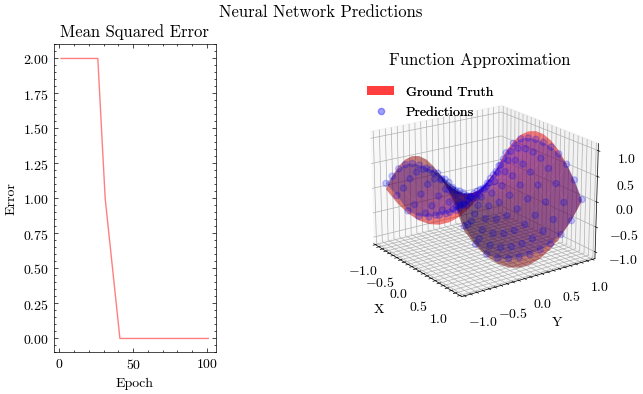
\includegraphics[width=\textwidth]{combined_files/combined_200_1.png}
    \end{center}
    { \hspace*{\fill} \\}

    % Add a bibliography block to the postdoc

    \bibliographystyle{IEEEtran}
\bibliography{references}
    
    
\end{document}
